\documentclass[dsc,numbers]{coppe}
\usepackage[utf8]{inputenc}
\usepackage{amsmath,amssymb}
\usepackage{hyperref}
\usepackage{siunitx}
\usepackage{booktabs}
\usepackage{cleveref}
\usepackage{minted}
\usepackage[section]{placeins}

%tikz
\usepackage{tikz}
\usetikzlibrary{shapes,arrows}

\makelosymbols
\makeloabbreviations

\begin{document}
  \title{Trabalho - Identificação de Sistemas}
  \foreigntitle{Thesis Title}
  \author{Raphael Timbó}{Silva}
  \advisor{Prof.}{Daniel}{Castello}
  
  \department{PEM}
  \date{01}{2017}

  \keyword{Primeira palavra-chave}
  \keyword{Segunda palavra-chave}
  \keyword{Terceira palavra-chave}

  \maketitle

%  \frontmatter
%  \dedication{A algu\'em cujo valor \'e digno desta dedicat\'oria.}


%  \chapter*{Agradecimentos}

Gostaria de agradecer a todos.

%  \begin{abstract}

Apresenta-se, nesta tese, ...

\end{abstract}


%  \begin{foreignabstract}

In this work, we present ...

\end{foreignabstract}


  \tableofcontents
  \listoffigures
  \listoftables
  \printlosymbols
  \printloabbreviations


  \mainmatter
  \chapter{Introdução}

O presente trabalho tem por objetivo apresentar os resultados e conclusões referentes ao projeto final da disciplina Identificação de Sistemas.

O trabalho consiste na análise de um sistema através do projeto de um filtro adaptativo \abbrev{FIR}{Finite Impulse Response} FIR (Finite Impulse Response). 

\section{Sistema utilizado}

O sistema utilizado é mostrado na \cref{fig:sistema}. 

\begin{figure}[!h]
	\centering
	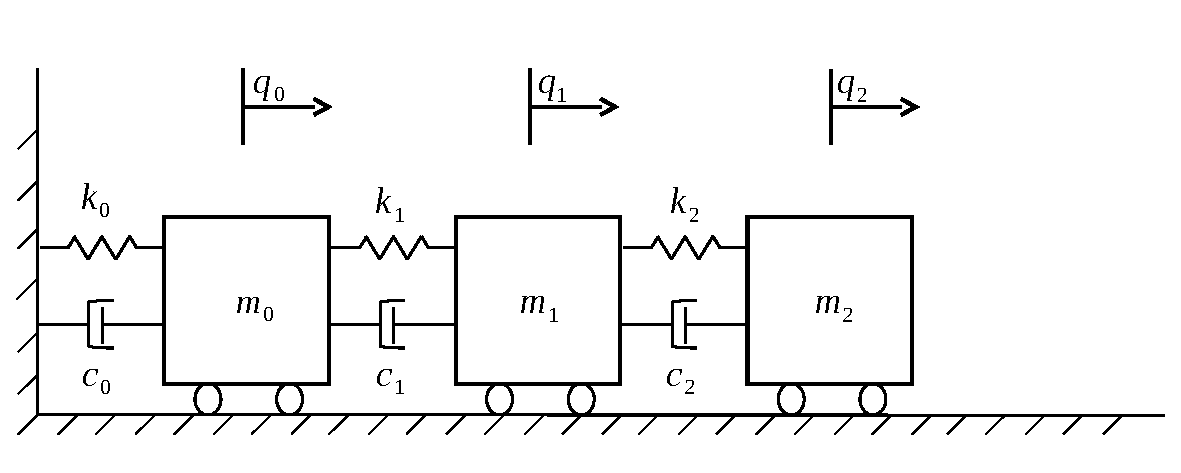
\includegraphics[width=0.8\textwidth]{IMGS/sistema.pdf}
	\caption{Sistema utilizado na análise.}
	\label{fig:sistema}
\end{figure}

Para este sistema temos que a energia cinética é:

\begin{equation}
T 
= \frac{1}{2}[m_0\dot{q_0}(t)^2 + m_1\dot{q_1}(t)^2 + m_2\dot{q_2}(t)^2] 
= \frac{1}{2}{\bf \dot{q}}^T(t)M{\bf \dot{q}}(t)
\end{equation}
onde 
\begin{equation*}
{\bf q(t)} = [q_0(t) \  q_1(t) \ q_2(t)]^T
\end{equation*}
é o vetor de configuração e
\begin{equation*}
M = 
\begin{bmatrix} 
m_0 & 0 & 0\\
0 & m_1 & 0 \\
0 & 0 & m_2
\end{bmatrix}
\end{equation*}  
é a matriz de massa do sistema.

A energia potencial tem a expressão:
\begin{equation}
\begin{split}
V &= \frac{1}{2}[k_0 q_0(t)^2 + k_1(q_1(t) - q_0(t))^2 + k_2 q_2(t)^2] \\
&= \frac{1}{2}[(k_0+k_1)q_0(t)^2 + (k_1+k_2)q_1(t)^2 + (k_2)q_2(t)^2 -2k_1  q_0(t)q_1(t) - 2k_2 q_2(t) \\
&= \frac{1}{2}{\bf \dot{q}}^T(t) K  {\bf \dot{q}}(t)
\end{split}
\end{equation}

onde
\begin{equation*}
K = 
\begin{bmatrix} 
k_0 +k_1 & -k_1 & 0\\
-k_1 & k_1+k_2 & -k_2 \\
0 & -k_2 & k_2
\end{bmatrix}
\end{equation*}   
é a matriz de rigidez do sistema.

Para o sistema utilizado temos que $m_i = 1 \ kg$ e $k_i = 1600 \ N/m$.

O amortecimento utilizado será o proporcional: $C = \alpha M + \beta K$. Iremos analisar o caso em que $\alpha = 10^{-3}$ e $\beta = 10^{-3}$.

\section{Resposta do sistema}

O sistema em questão possui a resposta \abbrev{FRF}{Função de Resposta em Frequência} FRF (Função de Resposta em Frequência) apresentada na \cref{fig:FRF_all}

\begin{figure}[!h]
	\centering
	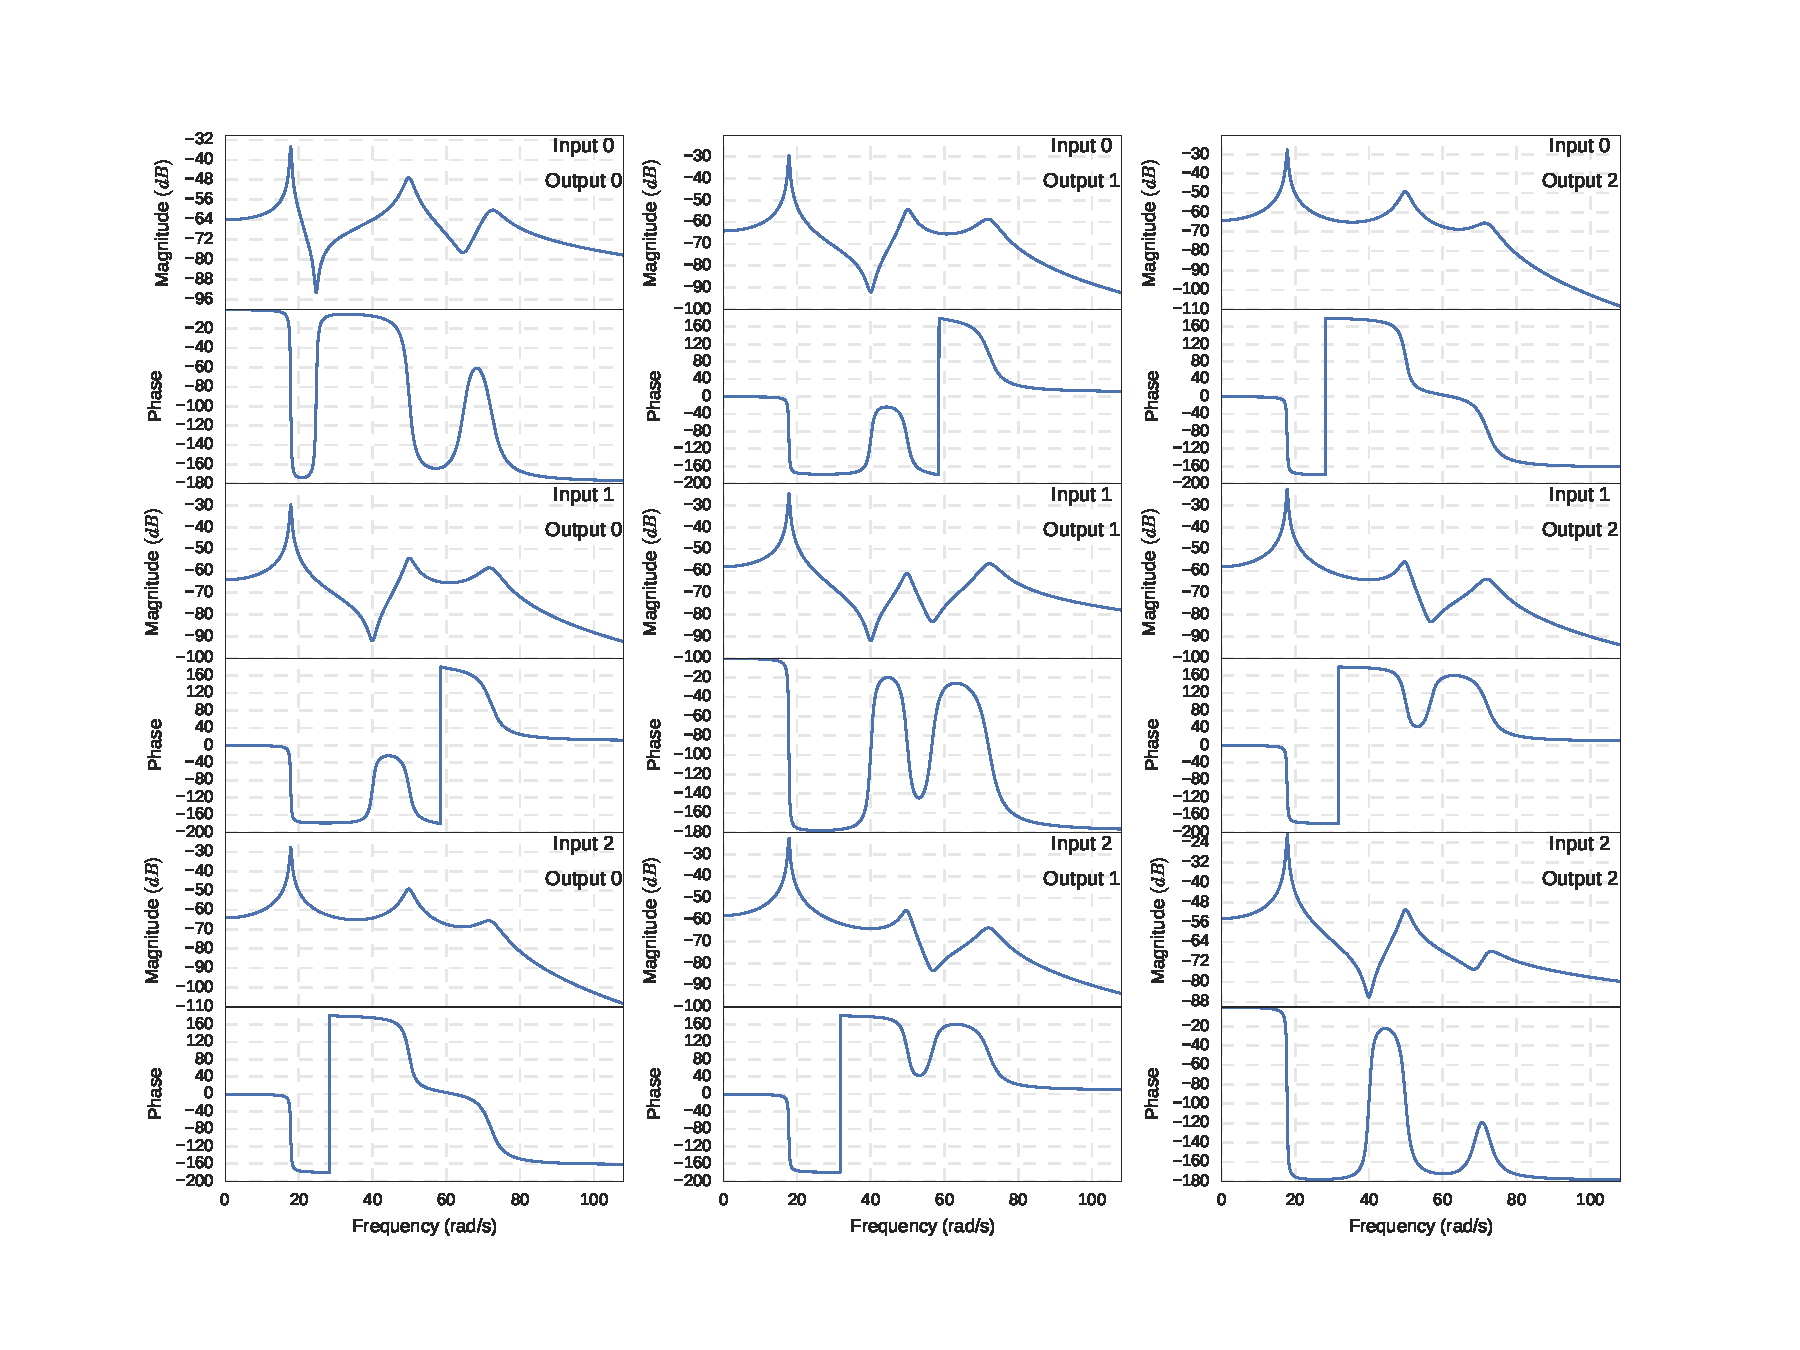
\includegraphics[trim={2.5cm, 1cm, 2.5cm, 2.5cm}, scale=0.55]{IMGS/FRF_all}
	\caption{FRF para o sistema em análise.}
	\label{fig:FRF_all}
\end{figure}

Para nossa análise iremos considerar uma força aplicada na massa 2 ($m_2$) e a medição nesta mesma massa, conforme ilustrado na \cref{fig:sistemaf}. A aplicação da força nessa massa corresponde à FRF que pode ser visualizada no canto inferior direito (input=2 e output=2). A FRF em questão é também mostrada na \cref{fig:FRF_i2_o2}

\begin{figure}
	\centering
	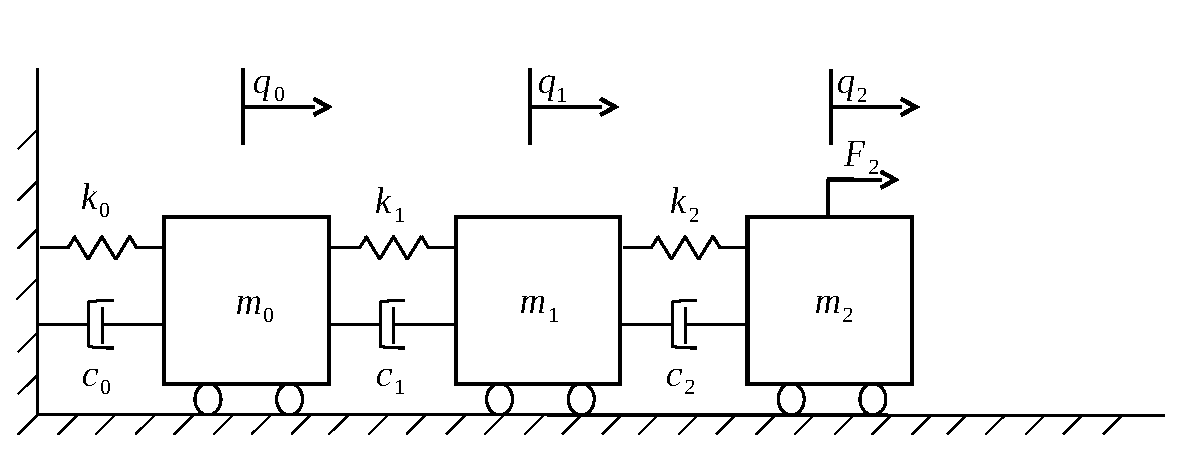
\includegraphics[width=0.8\textwidth]{IMGS/sistemaf}
	\caption{Aplicação de força e medição na massa $m_2$.}
	\label{fig:sistemaf}
\end{figure}

\begin{figure}
	\centering
	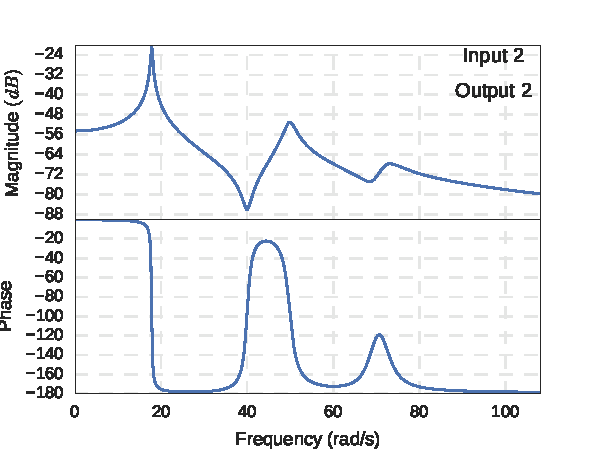
\includegraphics[scale=1]{IMGS/FRF_i2_o2}
	\caption{FRF para input em $m_2$ e medição em $m_2$.}
	\label{fig:FRF_i2_o2}
\end{figure}




  \chapter{Dados Pseudo-Experimentais}

\section{Resposta do sistema no tempo} \label{Resposta do sistema no tempo}

Para a construção dos dados pseudo-experimentais foram observados os seguintes casos:

Forçamento:
\begin{itemize}
	\item $F_0(t) = A_0 sin(2\pi f_0 t)$ 
	(Considere $\frac{\omega_1}{2\pi} \leq f_0 \leq \frac{\omega_2}{2\pi})$ 
	\item $F_1(t) = A_1 sin(2\pi f_1 t) + A_2 sin(2\pi f_2 t)$ 
	(Escolha 
	$\frac{0.8 \omega_1}{2\pi} \leq f_j \leq \frac{1.2 \omega_2}{2\pi}$ 
	e
	$A_2 = 2A_1$
	;
	$ j = 1, 2)$
	\item $F_2(t) = $ ruído branco
\end{itemize}

Número de amostras $N$:
\begin{itemize}
	\item $N = 1000$
	\item $N = 5000$
\end{itemize}

Valores para a relação entre sinal e ruído - \abbrev{SNR}{Signal to Noise Ratio} SNR (Signal to Noise Ratio):
\begin{itemize}
	\item $SNR = 90$
	\item $SNR = 50$
	\item $SNR = 10$
\end{itemize}

A \cref{fig:FRF_i2_o2_freq34} mostra a posição da frequência de excitação para a aplicação da força $F_0$, em que uma amplitude $A_0 = 1$ foi utilizada.

\begin{figure}
	\centering
	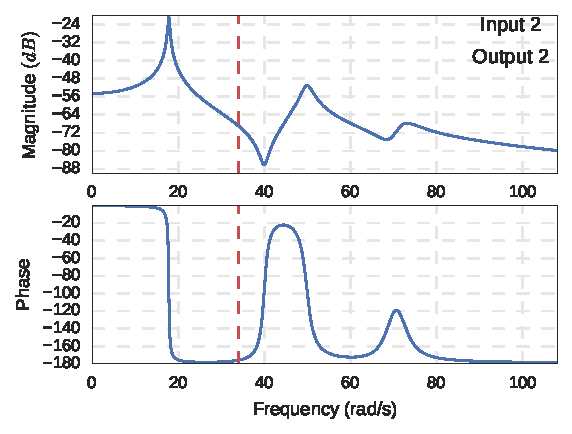
\includegraphics[scale=1]{FRF_i2_o2_freq34.pdf}
	\caption{Frequência de excitação para a força $F_0$.}
	\label{fig:FRF_i2_o2_freq34}
\end{figure}

A \cref{fig:F0_1000_tempo} mostra a resposta no tempo do sistema ao aplicarmos a força $F_0$ na frequência mostrada na \cref{fig:FRF_i2_o2_freq34} para uma amostragem $N = 1000$. Podemos observar que, para $N=1000$, temos uma excitação de aproximadamente 16 segundos e ainda temos algum transiente na resposta no tempo. Também é possível observar que essa parcela apresenta mais que uma frequência de oscilação.

\begin{figure}
	\centering
	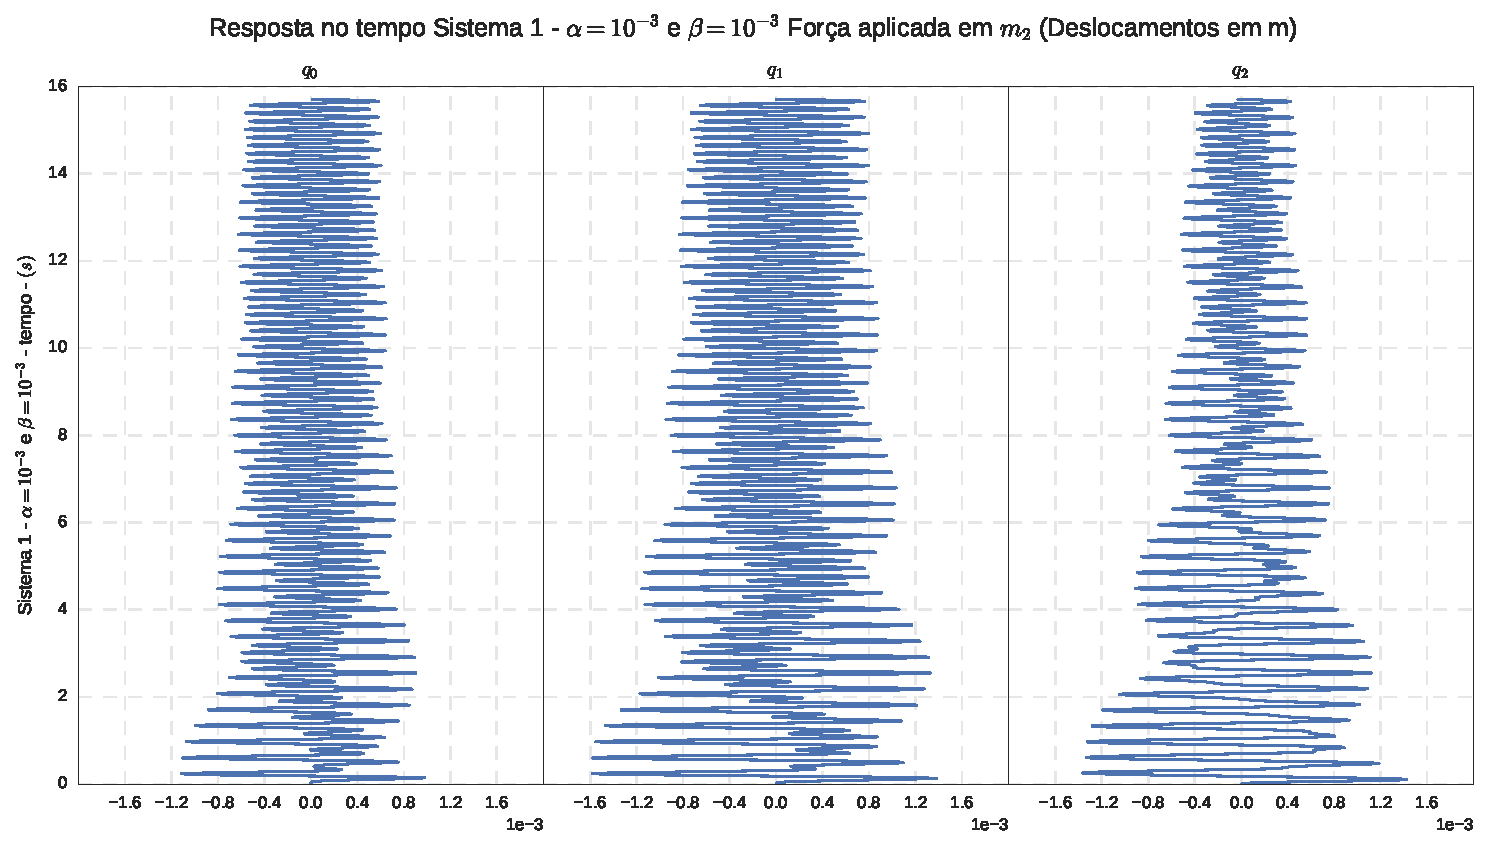
\includegraphics[scale=0.6]{F0_1000_tempo.pdf}
	\caption{Resposta no tempo para a força $F_0$ com $N=1000$.}
	\label{fig:F0_1000_tempo}
\end{figure}

A \cref{fig:F0_5000_tempo} mostra a resposta no tempo para $N=5000$. Neste caso, o tempo vai até aproximadamente 80 segundos e podemos observar que a parcela transiente é praticamente inexistente após os 20 segundos de excitação. Após esse tempo, é esperado que o sistema oscile apenas na frequência de excitação.

\begin{figure}
	\centering
	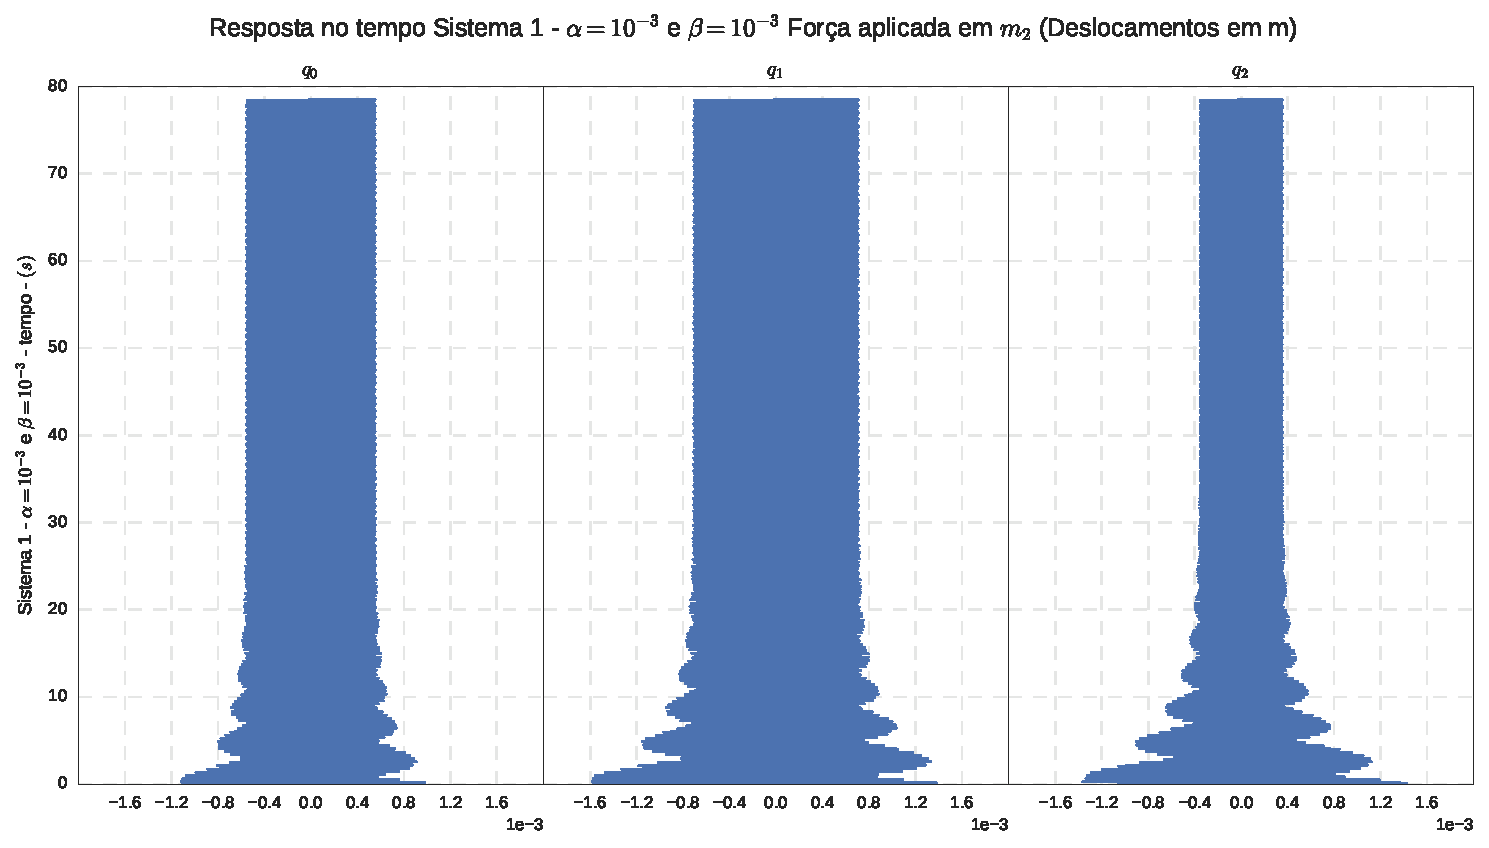
\includegraphics[scale=0.6]{F0_5000_tempo.pdf}
	\caption{Resposta no tempo para a força $F_0$ com $N=5000$.}
	\label{fig:F0_5000_tempo}
\end{figure}

Para a força $F_1$ a \cref{fig:FRF_i2_o2_freq_1_2} mostra as frequências de excitação que foram aplicadas na massa $m_2$. Podemos notar que nesse caso as forças aplicadas estão próximas as frequências naturais do sistema.

\begin{figure}
	\centering
	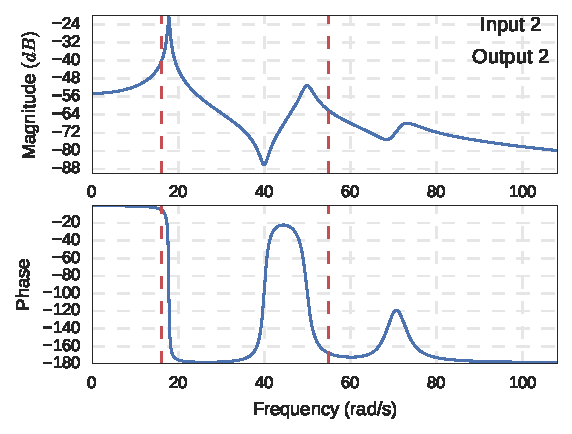
\includegraphics[scale=1]{FRF_i2_o2_freq_1_2.pdf}
	\caption{Frequência de excitação para a força $F_1$.}
	\label{fig:FRF_i2_o2_freq_1_2}
\end{figure}

A \cref{fig:F1_5000_tempo} mostra a resposta no tempo para $F_1$ com $ A_1 = 1 $, $ A_2 = 2  $ e $ N=5000 $. Como esperado, notamos um aumento na amplitude de \SI{1e-3}{\m} para \SI{1e-2}{\m} quando comparado à força $ F_0 $.

\begin{figure}
	\centering
	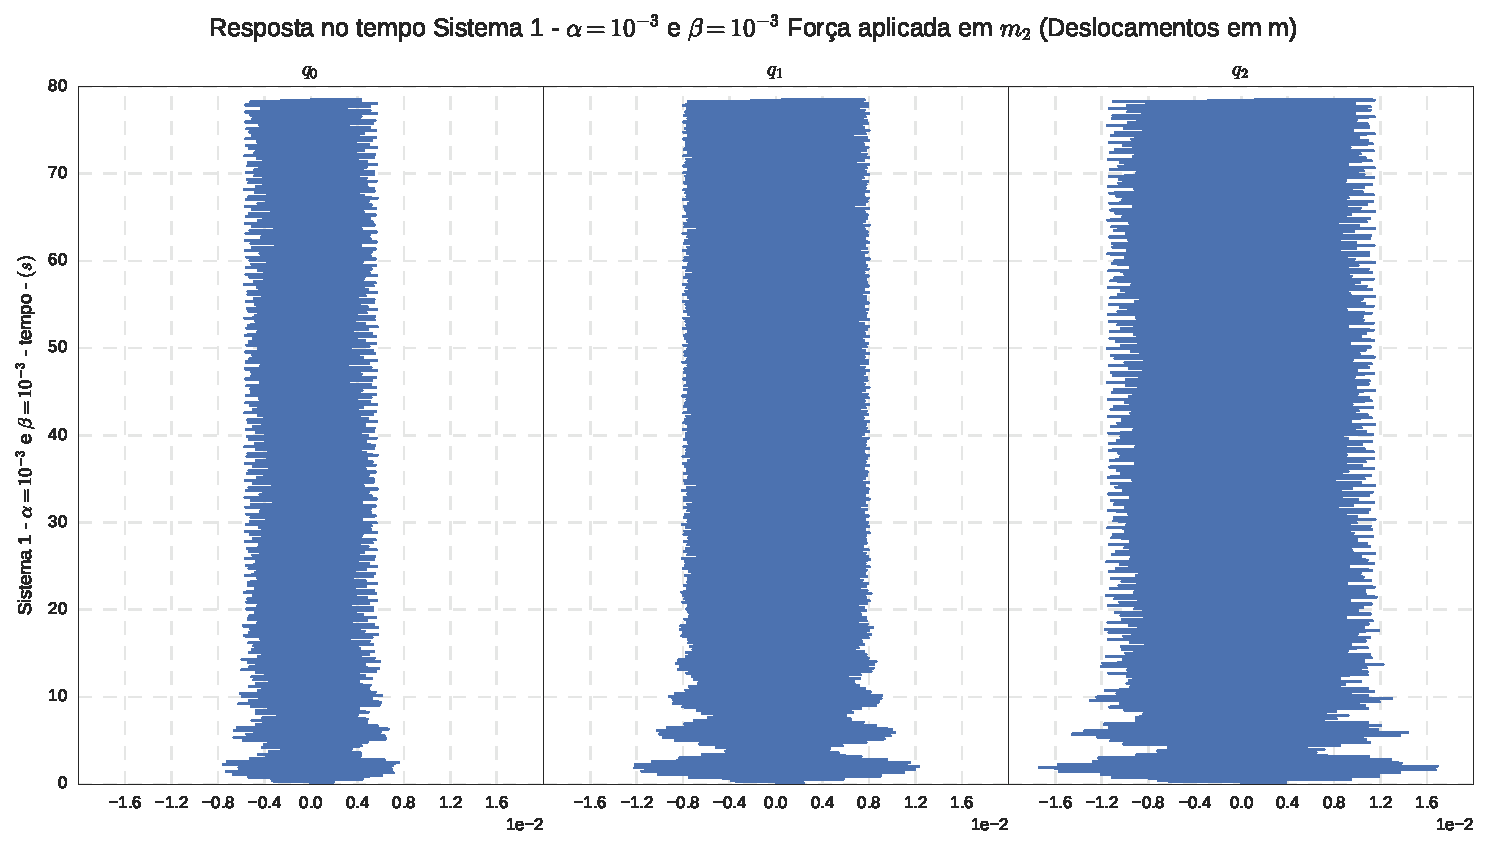
\includegraphics[scale=0.6]{F1_5000_tempo.pdf}
	\caption{Resposta no tempo para a força $F_1$ com $N=5000$.}
	\label{fig:F1_5000_tempo}
\end{figure}

O último caso de forçamento é mostrado na \cref{fig:F2_5000_tempo} onde um ruído branco com variância 1 é aplicado ao sistema.

\begin{figure}
	\centering
	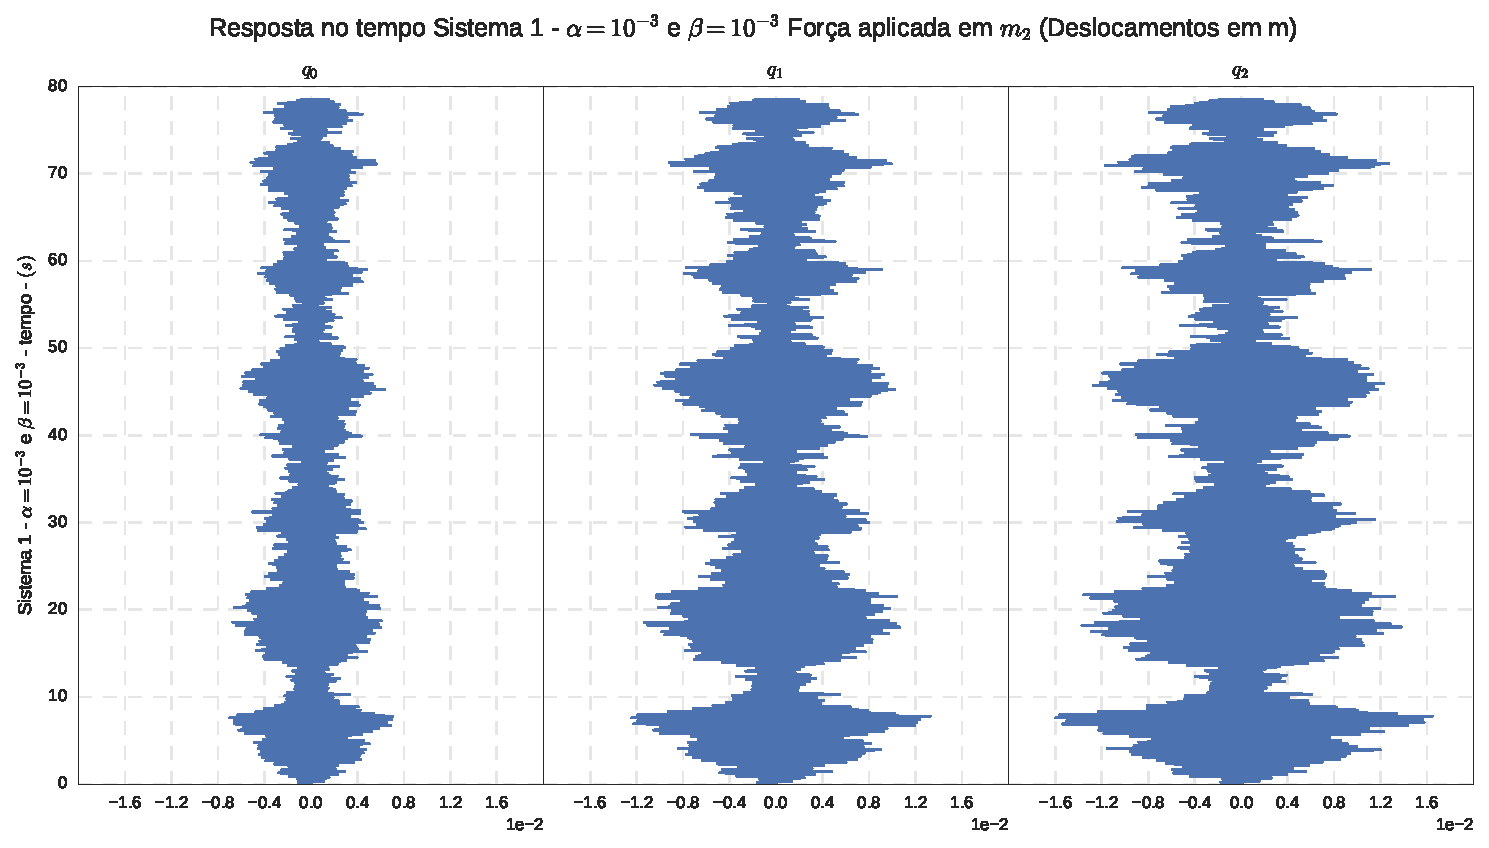
\includegraphics[scale=0.6]{F2_5000_tempo.pdf}
	\caption{Resposta no tempo para a força $F_2$ com $N=5000$.}
	\label{fig:F2_5000_tempo}
\end{figure}

\section{Adição do ruído}

Conforme mostrado no item \ref{Resposta do sistema no tempo}, a análise será feita para três diferentes níveis de ruído ($ SNR $ = 90, 50, 10). 

Temos então que o sinal utilizado para o projeto do filtro será:

\begin{equation}
y = y^{ideal} + n
\end{equation}
onde $ n $ representa um ruído inserido no sinal.

Para calcularmos a amplitude do ruído inserido '$ n $' utilizaremos a \cref{eq:snr}.

\begin{equation} \label{eq:snr}
SNR = 20log_{10}\Bigg(\frac{A_s}{A_n}\Bigg) \rightarrow A_n = \frac{A_s}{10^{SNR/20}}
\end{equation}

Abaixo (\cref{fig:F0_noise_90}, \cref{fig:F0_noise_10} e \cref{fig:F2_noise_10}), são mostrados alguns resultados comparando o sinal puro e o sinal corrompido para um determinado nível de ruído.

\begin{figure}
	\centering
	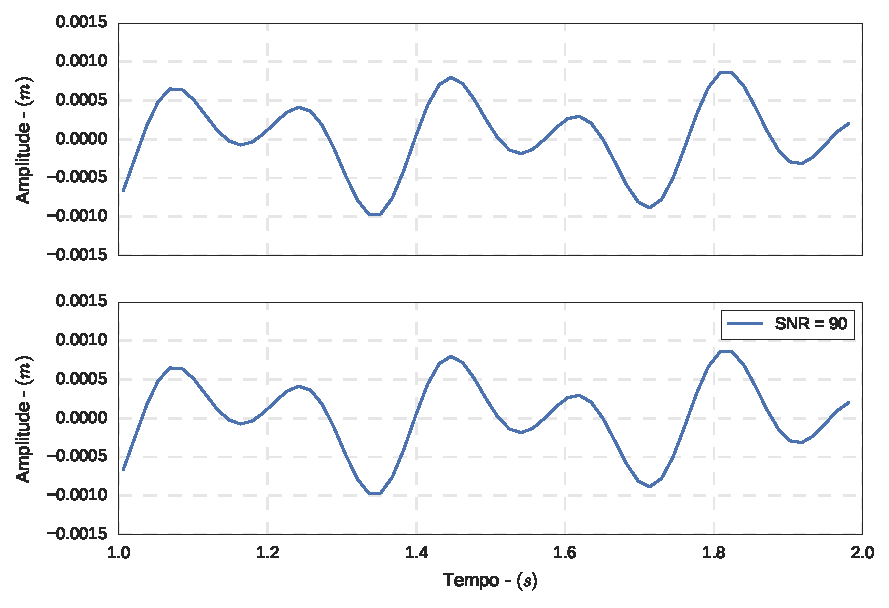
\includegraphics[scale=0.6]{F0_noise_90}
	\caption{Sinal puro e sinal corrompido para $ F_0 $ e $ SNR=90 $.}
	\label{fig:F0_noise_90}
\end{figure}

\begin{figure}
	\centering
	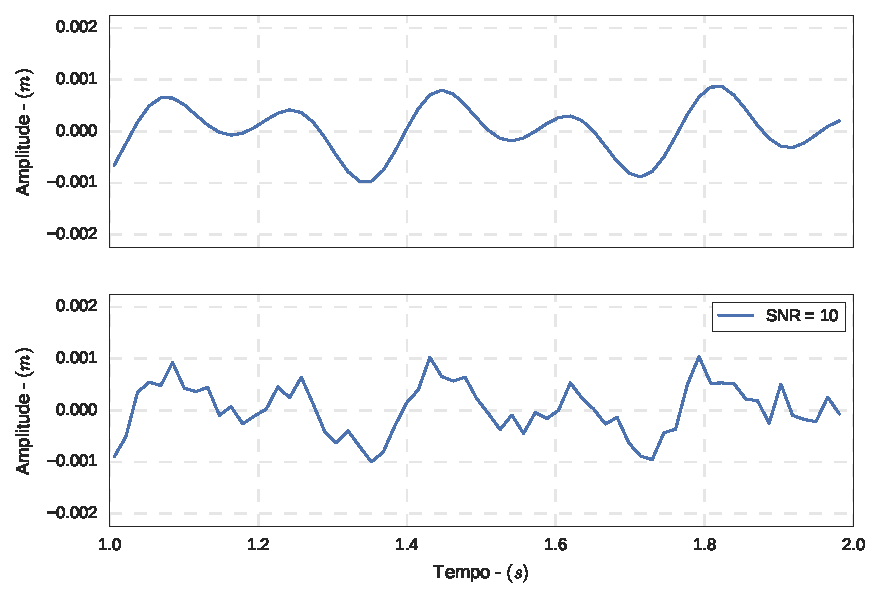
\includegraphics[scale=0.6]{F0_noise_10}
	\caption{Sinal puro e sinal corrompido para $ F_0 $ e $ SNR=10 $.}
	\label{fig:F0_noise_10}
\end{figure}

\begin{figure}
	\centering
	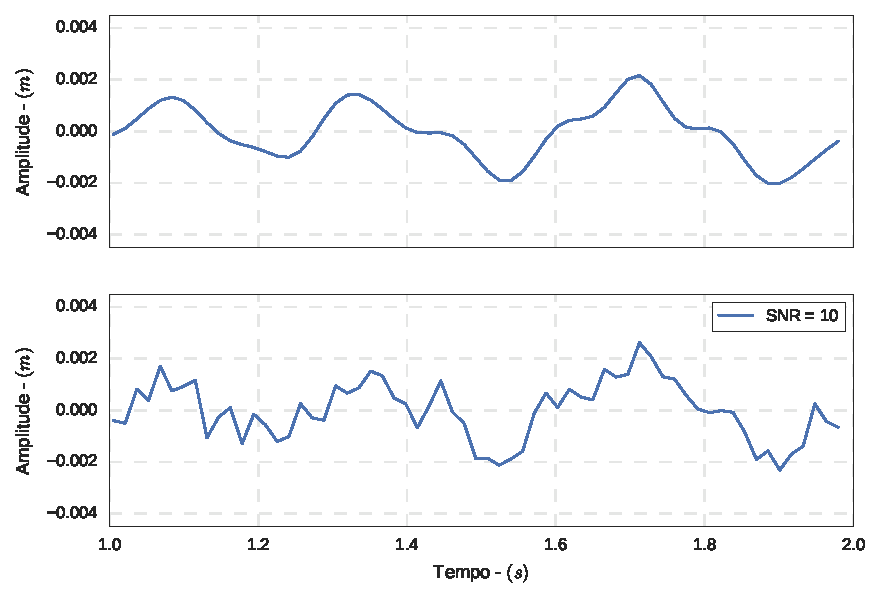
\includegraphics[scale=0.6]{F2_noise_10}
	\caption{Sinal puro e sinal corrompido para $ F_2 $ e $ SNR=10 $.}
	\label{fig:F2_noise_10}
\end{figure}


  \chapter{Projeto do Filtro Adaptativo}

Para o algoritmo do filtro adaptativo \citet{castello2005experimental} apresentam algumas opções que podem ser utilizadas. No caso do presente trabalho o algoritmo \abbrev{LMS}{Least Mean Squares} LMS (Least Mean Squares) foi escolhido.

\section{Algoritmo LMS}

Como mostrado por \citet{diniz1997adaptive}, a configuração normalmente aplicada para identificação de sistemas com filtros adaptativos é mostrada na \cref{fig:config_filtro}. Nesta configuração temos que $ x(k) $ é o sinal de entrada, o sinal de saída do sistema que desejamos identificar é $ d(k) $ e a saída do filtro é $ y(k) $. Estes sinais são comparados e o erro $ e(k) $ é calculado. 
 
\begin{figure}[h]
	\centering
	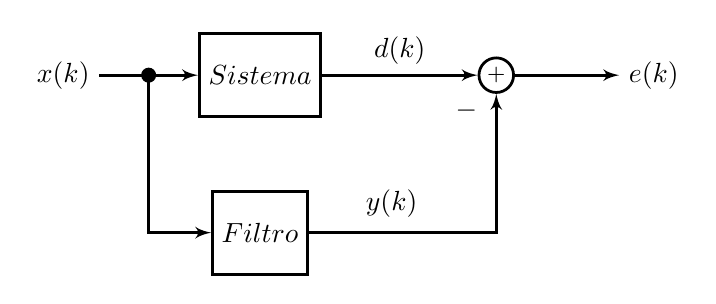
\begin{tikzpicture}[auto,>=latex']
	\tikzstyle{block} = [draw, shape=rectangle, minimum height=3em, minimum width=3em, node distance=2cm, line width=1pt]
	\tikzstyle{sum} = [draw, shape=circle, node distance=3cm, line width=1pt, minimum width=1.25em]
	\tikzstyle{branch}=[fill,shape=circle,minimum size=2pt,inner sep=0pt]
	%Creating Blocks and Connection Nodes
	\node at (-2.5,0) (input) {$x(k)$};
	\node [block] (sistema) {$Sistema$};
	\node [sum, right of=sistema, label=-120:$ - $] (sum) {};
	\node at (sum) (plus) {{\footnotesize$+$}};
	\node at (5,0) (output) {$e(k)$};
	\path (sistema) -- coordinate (med) (sum);
	\path (input) -- coordinate(branch1) (sistema);
	\node [block, below of=sistema, label={[label distance=0.6cm]3:$ y(k) $}] (filtro) {$Filtro$};
	%Conecting Blocks
	\begin{scope}[line width=1pt]
	\draw[->] (input) -- (sistema);
	\draw[->] (sistema) to node {$ d(k) $} (sum);
	\draw[->] (sum) -- (output);
	\draw[->] (branch1) node[branch] {-} |- (filtro);
	\draw[->] (filtro) -| (sum);
	\end{scope}
	\end{tikzpicture}
	\caption{Configuração utilizada no algoritmo para filtros adaptativos.}
	\label{fig:config_filtro}
\end{figure}

Os valores de saída do filtro são calculados a partir de uma combinação linear dos seus coeficientes e do sinal de entrada, isto é:

\begin{equation}\label{eq:y}
y(k) = \sum_{i=0}^{N} w_i(k) x_i(k) = {\bf w}^T(k) {\bf x}(k)
\end{equation}
onde ${\bf w}(k)$ representa os coeficientes do filtro.

Para aplicações onde o vetor do sinal de entrada é uma versão atrasada do mesmo sinal, isto é: $x_0(k) = x(k),x_1(k) = x(k - 1),...,x_N(k) = x(k - N)$, $y(k)$ é o resultado da aplicação de um filtro FIR ao sinal de entrada $x(k)$. Neste caso temos:

\begin{equation}
y(k) = \sum_{i=0}^{N} w_i(k) x(k-i) = {\bf w}^T(k) {\bf x}(k)
\end{equation}

onde ${\bf x}(k) = [x(k) \ x(k-1) \ ... \ x(k - N)]^T$.

O \abbrev{MSE}{Mean Square Error} MSE (Mean Square Error) pode ser calculado como:

\begin{equation} \label{eq:mse1}
\xi(k) = E[e^2(k)] = E[d^2(k) - 2d(k)y(k) + y^2(k)]
\end{equation}

Podemos reescrever a \cref{eq:mse1}:

\begin{equation}
\xi = E[d^2(k)] - 2{\bf w}^T{\bf p} + {\bf w}^T {\bf Rw}
\end{equation}

onde $p = E[d(k){\bf x}(k)]$ é o vetor de correlação cruzada entre o sinal desejado e o sinal de entrada e ${\bf R} = E[{\bf x}(k){\bf x}^T(k)]$ é a matriz de correlação do sinal de entrada.

Se ${\bf p}$ e ${\bf R}$ são conhecidos, podemos encontrar a solução para ${\bf w}$ que minimiza $\xi$.

O gradiente do MSE relativo aos coeficientes é:

\begin{equation}
{\bf g_w} = \frac{\partial \xi}{\partial {\bf w}} = 
\Bigg[\frac{\partial \xi}{\partial {w_0}}
\frac{\partial \xi}{\partial {w_1}} ...
\frac{\partial \xi}{\partial {w_N}}
\Bigg] = -2{\bf p} + 2{\bf Rw}
\end{equation}

Igualando o gradiente a zero encontramos o vetor de coeficientes que minimiza $\xi$:

\begin{equation}
{\bf w}_0 = {\bf R}^{-1}{\bf p}
\end{equation}

Se boas estimativas ${\bf \hat{p}}$ e ${\bf \hat{R}}$ estão disponíveis podemos buscar uma solução:

\begin{align}
{\bf w}(k+1) & = {\bf w}(k) - \mu {\bf \hat{g}_w}(k) \\
& = {\bf w}(k) + 2 \mu ({\bf \hat{p}}(k) - {\bf \hat{R}}(k){\bf w}(k))
\end{align}

para $k = 0, 1, 2,...,$ onde ${\bf \hat{g}_w}(k)$ representa uma estimativa do gradiente da função objetivo com respeito aos coeficientes do filtro.

Uma possível solução é estimar o gradiente com estimativas instantâneas de ${\bf R}$ e de ${\bf p}$.

\begin{align}
& {\bf \hat{R}}(k) = {\bf x}(k) {\bf x}^T(k) \\
& {\bf \hat{p}}(k) = d(k)       {\bf x}(k)
\end{align}

Temos então que a estimativa para o gradiente é:

\begin{equation}
{\bf \hat{g}_w}(k) = -2e(k){\bf x}(k)
\end{equation}

Chegamos então ao algoritmo LMS em que a equação de atualização é:

\begin{equation}\label{eq:LMS}
{\bf w}(k+1) = {\bf w}(k) + 2 \mu e(k) {\bf x}(k)
\end{equation}

onde o fator de convergência $\mu$ deve ser escolhido em um range que garanta a convergência.

\section{Implementação do filtro}

O filtro será implementado em Python como explicado abaixo.

Uma classe \mintinline{python3}{class LMSFilter()} será criada para o filtro. Essa classe contém uma função de inicialização que possui como argumentos de entrada o número de coeficientes do filtro e o fator de convergência $\mu$. Na criação do filtro os coeficientes são igualados a zero como mostrado no código abaixo.

\begin{minted}{python3}
  class LMSFilter(object):
    def __init__(self, Nc, mu):
      """
      Iniciar filtro com Nc coeficientes.
      """
      self.Nc = Nc
      self.mu = mu
      # valores iniciais para o filtro w = [0, 0, ..., 0]
      self.w = np.zeros(Nc)
\end{minted}

O filtro possui uma função \mintinline{python3}{predict(self, x)} que calcula a saída prevista para o filtro baseado no sinal de entrada \mintinline{python}{x} $(x(k))$. O cálculo é feito conforme a \cref{eq:y}:

\begin{equation*}
y(k) = \sum_{i=0}^{N} w_i(k) x_i(k) = {\bf w}^T(k) {\bf x}(k) \tag{\ref{eq:y} revisitada}
\end{equation*}

\begin{minted}{python3}
  def predict(self, x):
    y = self.w @ x
    return y
\end{minted}

A atualização do filtro é feita pela função \mintinline{python3}{update(self, d, x)} considerando a \cref{eq:LMS}:

\begin{equation*}
{\bf w}(k+1) = {\bf w}(k) + 2 \mu e(k) {\bf x}(k) \tag{\ref{eq:LMS} revisitada}
\end{equation*}

\begin{minted}{python3}
  def update(self, d, x):
    """
    Atualizar filtro baseado no sinal de entrada x
    e no valor desejado d.
    """
    y = self.w @ x
    e = d - y
    self.w += 2*self.mu * e * x
\end{minted}
  \chapter{Resultados e Discussões}

\section{Resultados para $ F_0 $}\label{sec_F_0}
\subsection{Adaptação do filtro}

Os resultados da adaptação do filtro para uma força $F_0(t) = A_0 sin(2\pi f_0 t)$ com $ N=1000 $  e $ SNR = 90 $ são mostrados na \cref{fig:F0_1000_90_conv}. O número de coeficientes do filtro ($ N_c $) e o fator de convergência ($ \mu $) utilizados são apresentados na figura.

\begin{figure}[!h]
	\centering
	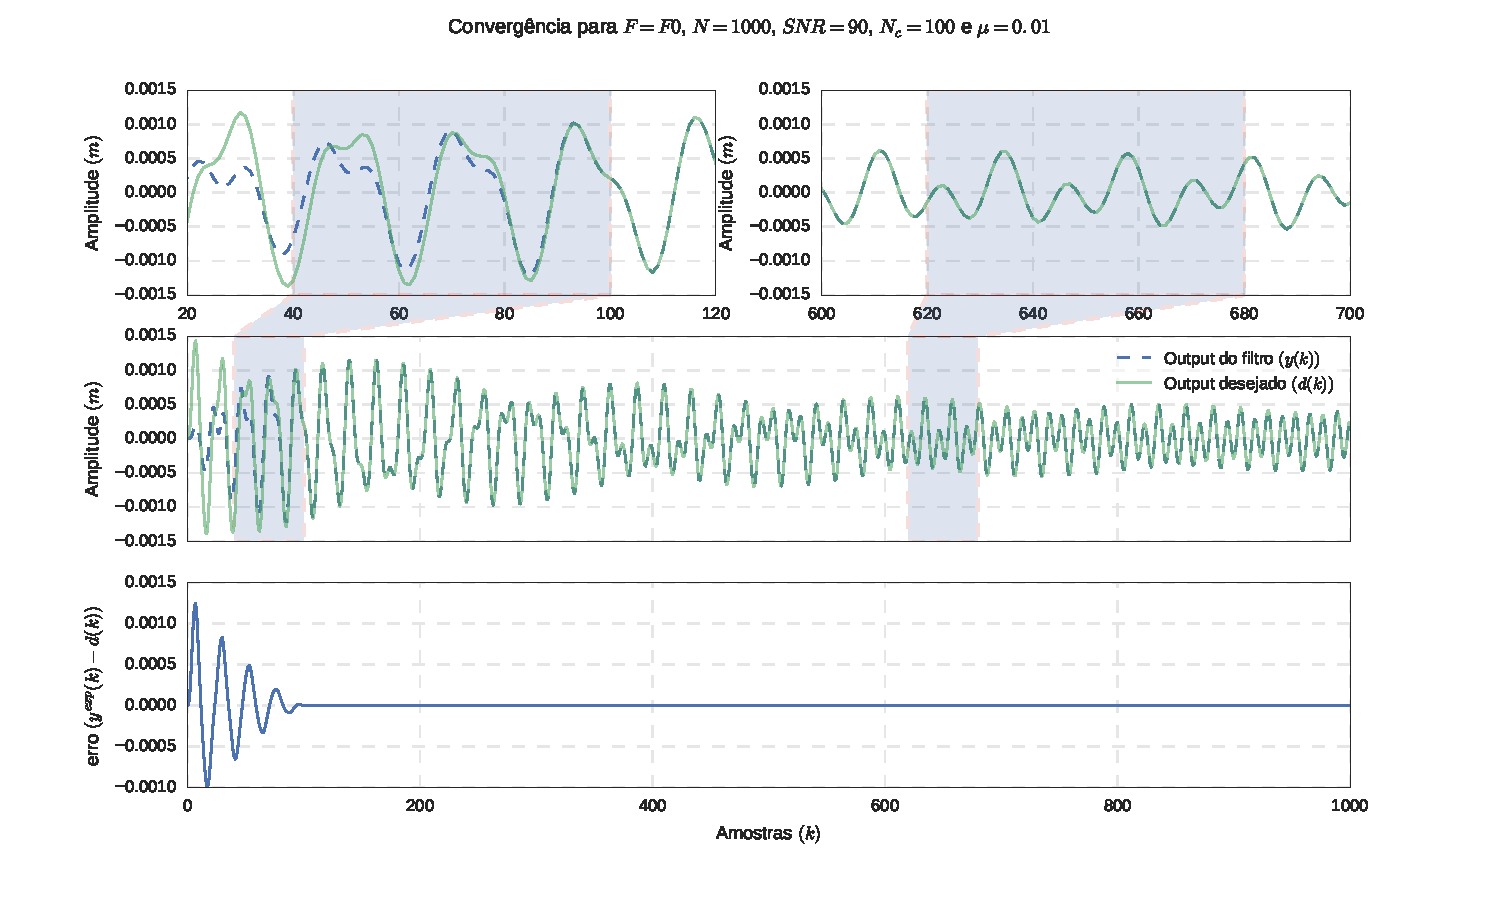
\includegraphics[scale=0.7]{F0_1000_90_conv}
	\caption{Evolução do filtro para $ F=F_0 $, $ N=1000 $ e $ SNR=90 $.}
	\label{fig:F0_1000_90_conv}
\end{figure}

Para o caso do seno puro podemos o filtro tem uma convergência rápida e com menos de 100 iterações o erro já é próximo de zero. 

Na \cref{fig:F0_1000_10_conv} são apresentados os resultados para $ N=1000 $ e $ SNR=10 $. Podemos observar que, mesmo com um nível de ruído mais elevado, o algoritmo apresentou uma convergência rápida.

\begin{figure}
	\centering
	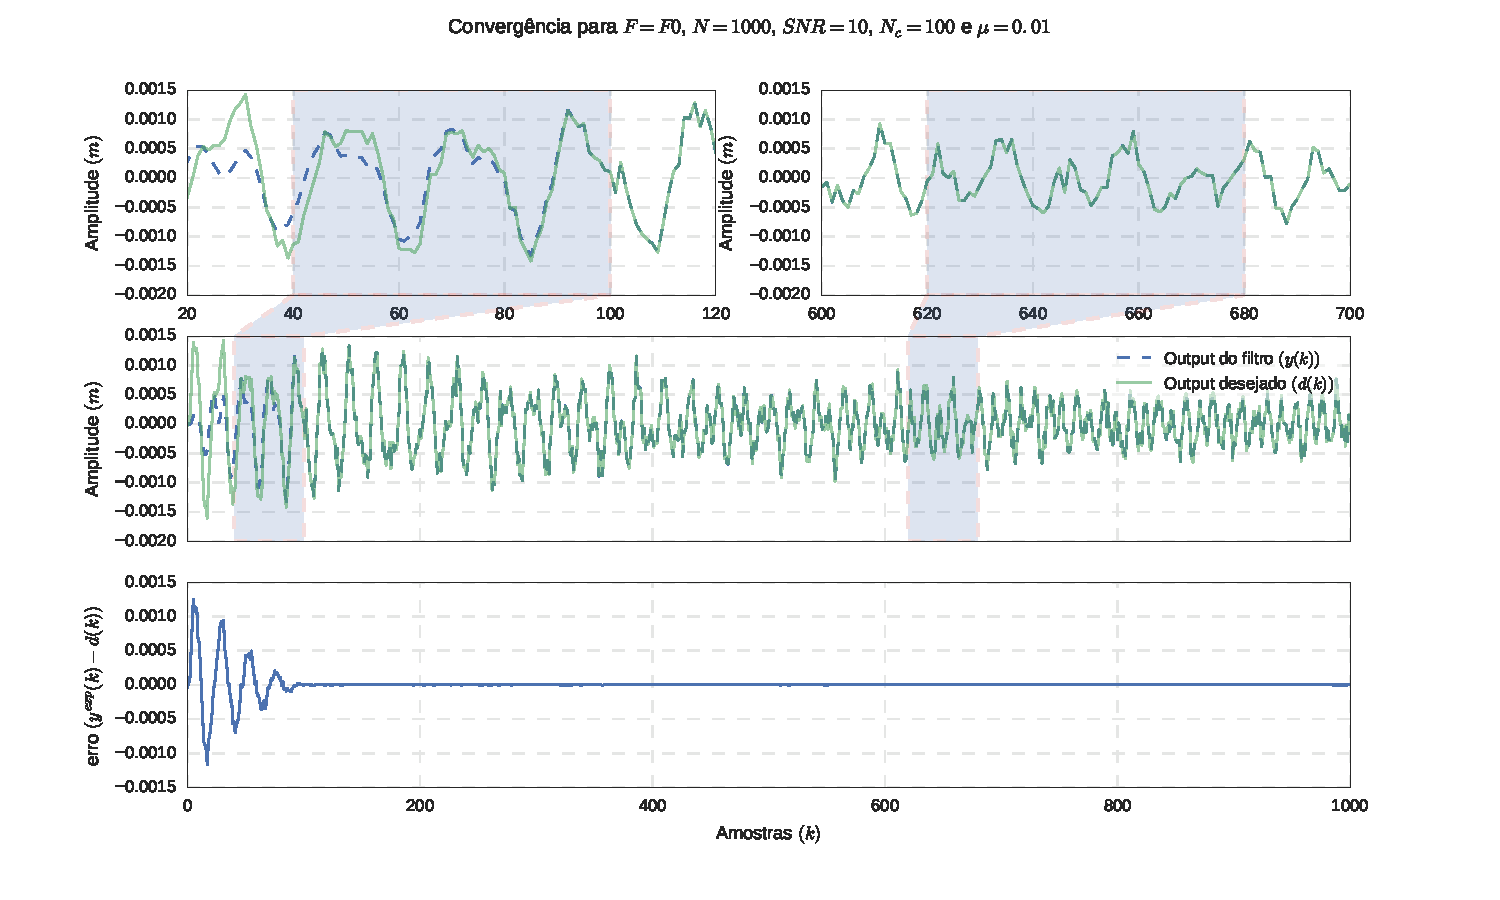
\includegraphics[scale=0.7]{F0_1000_10_conv}
	\caption{Evolução do filtro para $ F=F_0 $, $ N=1000 $ e $ SNR=10 $.}
	\label{fig:F0_1000_10_conv}
\end{figure}

\subsection{FRF do filtro}

Na \cref{fig:F0_1000_90_FRF_med_False} é apresentada a FRF do filtro obtido com $ SNR=90 $ considerando o último vetor de coeficientes, e na \cref{fig:F0_1000_90_FRF_med_True} é apresentada a FRF considerando o vetor obtido através do valor esperado dos coeficientes tomando por base as observações da segunda metade do vetor de dados. A \cref{fig:F0_1000_10_FRF} apresenta os resultados para $ SNR=10 $. 

Podemos observar que FRF do filtro obtido não apresenta bons resultados, aproximando-se do valor esperado apenas na frequência de excitação (\SI{34}{\radian \per \s}). Podemos notar um aumento na amplitude próxima à primeira frequência natural do sistema, mas o valor não se aproxima do esperado. Outro ponto importante é que, para este caso, a FRF do filtro não se mostrou sensível ao nível de ruído. A utilização do último vetor de coeficientes $ w $ ou do valor esperado para a segunda metade do vetor de dados também não teve impacto significativo na resposta. 

\begin{figure}
	\centering
	\begin{subfigure}{0.9\textwidth}
		\centering
		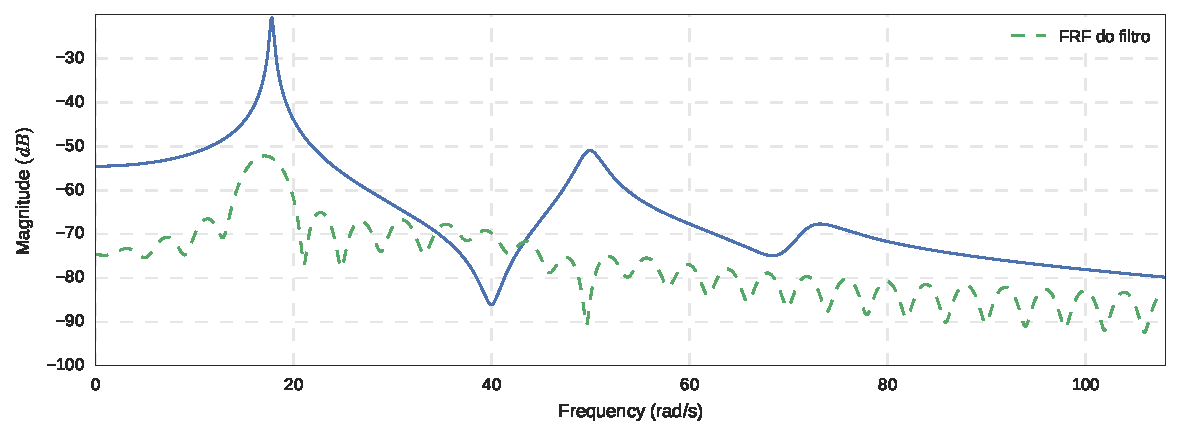
\includegraphics[width=0.9\linewidth]{F0_1000_90_FRF_med_False}
		\caption{último vetor $ w $}
		\label{fig:F0_1000_90_FRF_med_False}
	\end{subfigure}
	\begin{subfigure}{0.9\textwidth}
		\centering
		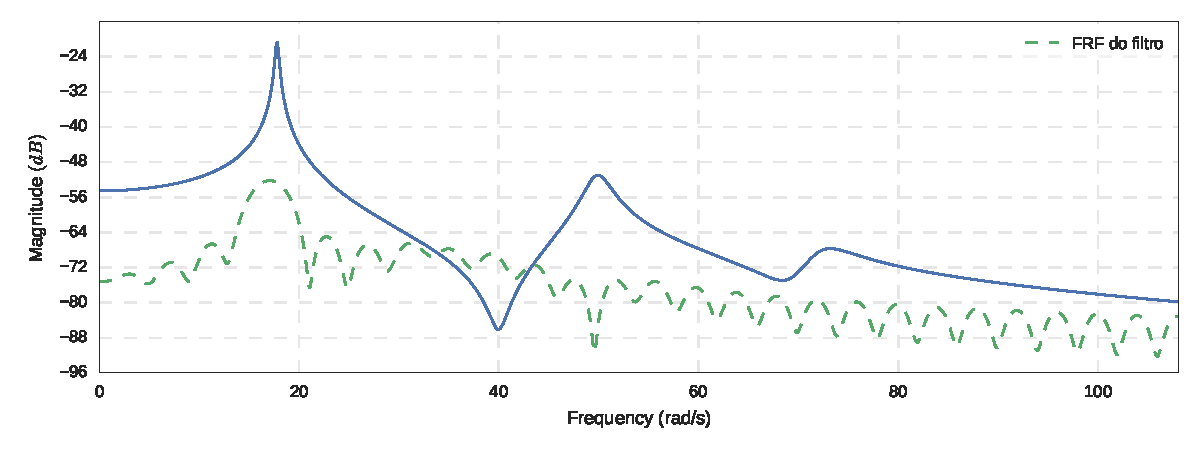
\includegraphics[width=0.9\linewidth]{F0_1000_90_FRF_med_True}
		\caption{valor médio de $ w $}
		\label{fig:F0_1000_90_FRF_med_True}
	\end{subfigure}
	\caption{FRF do filtro obtido para $ F=F_0 $, $ N=1000 $ e $ SNR=90 $.}
\end{figure}

\begin{figure}
	\centering
	\begin{subfigure}{0.9\textwidth}
		\centering
		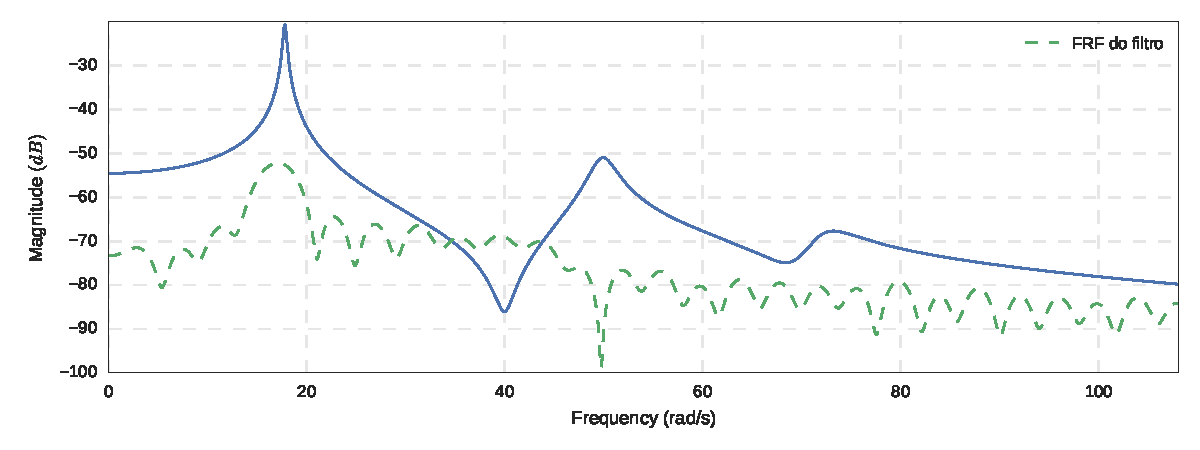
\includegraphics[width=0.9\linewidth]{F0_1000_10_FRF_med_False}
		\caption{último vetor $ w $}
		\label{fig:F0_1000_10_FRF_med_False}
	\end{subfigure}
	\begin{subfigure}{0.9\textwidth}
		\centering
		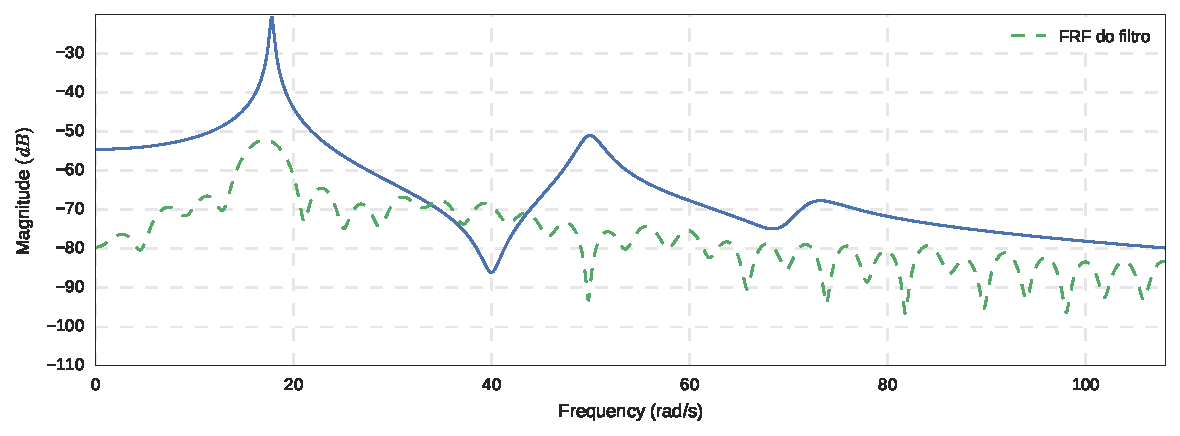
\includegraphics[width=0.9\linewidth]{F0_1000_10_FRF_med_True}
		\caption{valor médio de $ w $}
		\label{fig:F0_1000_10_FRF_med_True}
	\end{subfigure}
	\caption{FRF do filtro obtido para $ F=F_0 $, $ N=1000 $ e $ SNR=10 $.}
	\label{fig:F0_1000_10_FRF}
\end{figure}

\subsection{Predição}

Para analisarmos a predição do filtro, foi escolhida uma força arbitrária $ F_3 $ conforme \cref{eq:F_3}

\begin{equation}\label{eq:F_3}
F_3 = B_1 sin(\omega_1 t)
+ B_2 sin(\omega_2 t)
+ B_3 sin(\omega_3 t)
+ \nu
\end{equation}
onde $ B_1=\SI{1}{\N} $, $ B_2=\SI{2}{\N}$ , $ B_3=\SI{3}{\N} $, $ \omega_1= \SI{14}{\radian \per \s} $, $ \omega_2= \SI{40}{\radian \per \s} $, $ \omega_3= \SI{65}{\radian \per \s} $ e $ \nu $ é um ruído branco de variância 1.

A \cref{fig:F0_1000_90_pred} mostra a predição para o filtro obtido com $ F=F_0 $, $ N=1000 $ e $ SNR=90 $. Podemos observar que a predição obtida com o filtro não é boa e o erro ($ e(n)=y^{exp}(n) - y(n) $) é da ordem do valor previsto pelo filtro.

\begin{figure}[h]
	\centering
	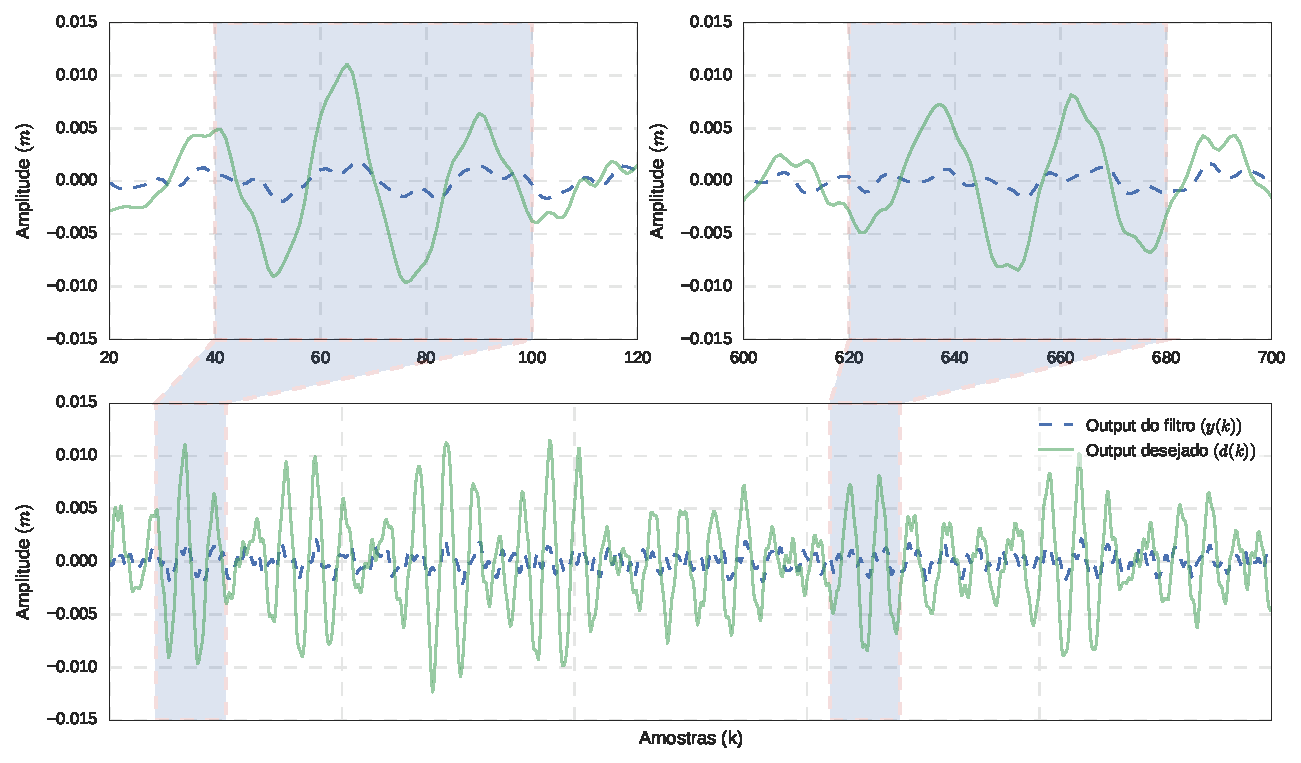
\includegraphics[scale=0.7]{F0_1000_90_pred}
	\caption{Predição do filtro obtido com $ F=F_0 $, $ N=1000 $ e $ SNR=90 $.}
	\label{fig:F0_1000_90_pred}
\end{figure}

Os resultados obtidos para os diferentes valores de $ N $ e $ SNR $ não apresentam diferença para o caso em que $ F=F_0 $ e por isso serão omitidos.

\section{Resultados para $ F_1 $}
\subsection{Adaptação do filtro}

Os resultados da adaptação do filtro para uma força $F_1(t) = A_1 sin(2\pi f_1 t) + A_2 sin(2\pi f_2 t)$  com $ N=1000 $  e $ SNR = 90 $ são mostrados na \cref{fig:F1_1000_90_conv}. Para este caso a convergência se mostrou próxima ao que foi obtido na análise de $ F_0 $. 

\begin{figure}
	\centering
	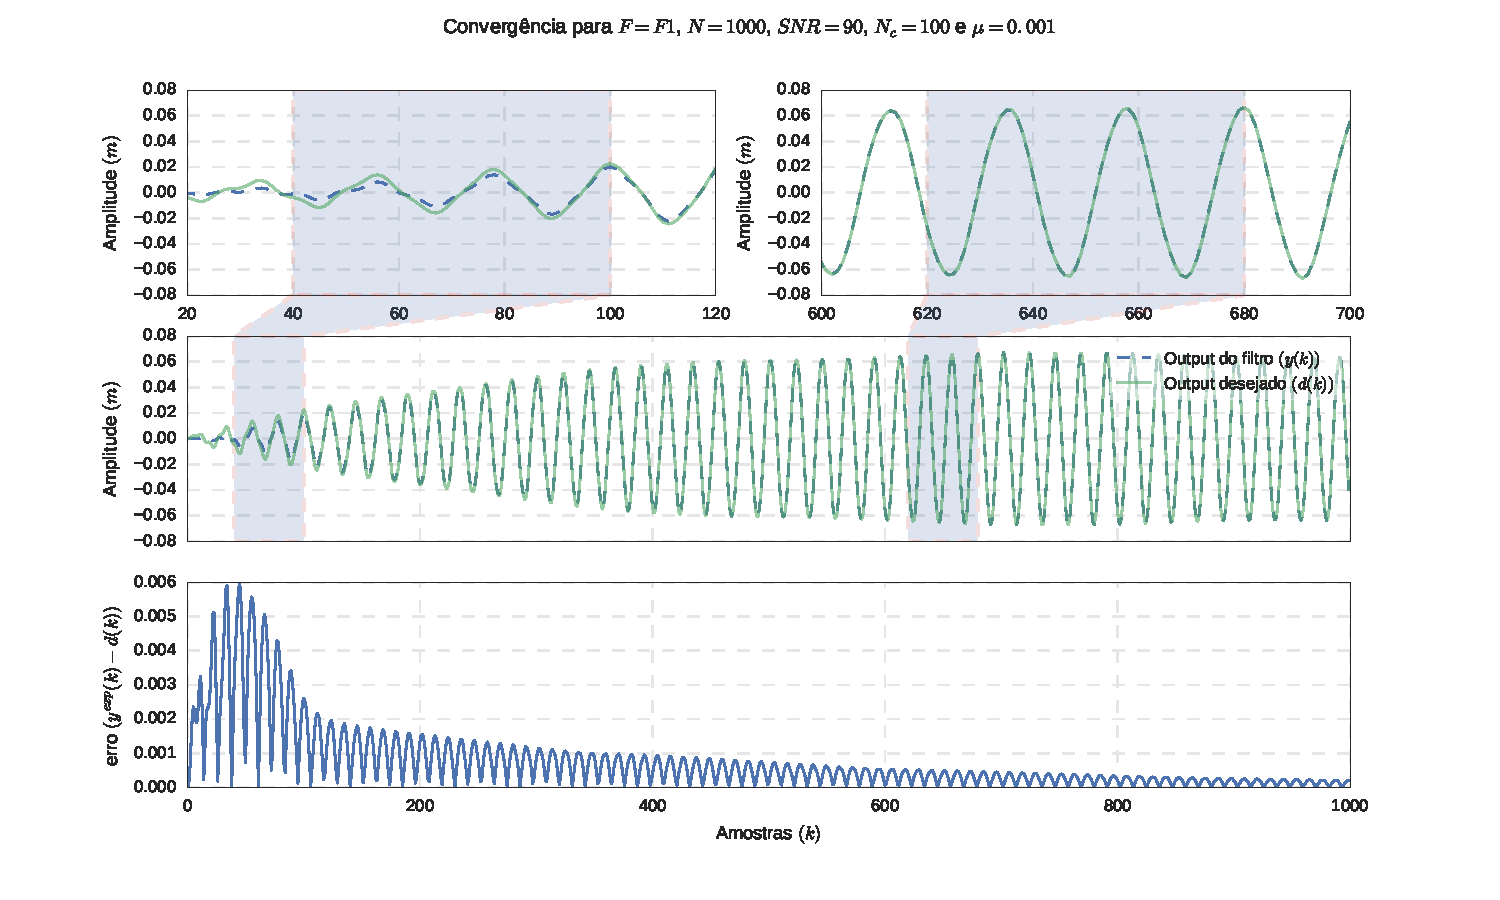
\includegraphics[scale=0.7]{F1_1000_90_conv}
	\caption{Evolução do filtro para $ F=F_1 $, $ N=1000 $ e $ SNR=90 $.}
	\label{fig:F1_1000_90_conv}
\end{figure}

Na \cref{fig:F1_1000_10_conv} são apresentados os resultados para $ N=1000 $ e $ SNR=10 $. Para este caso a convergência não é boa e ao fim das iterações o erro do filtro ainda é alto. 

\begin{figure}
	\centering
	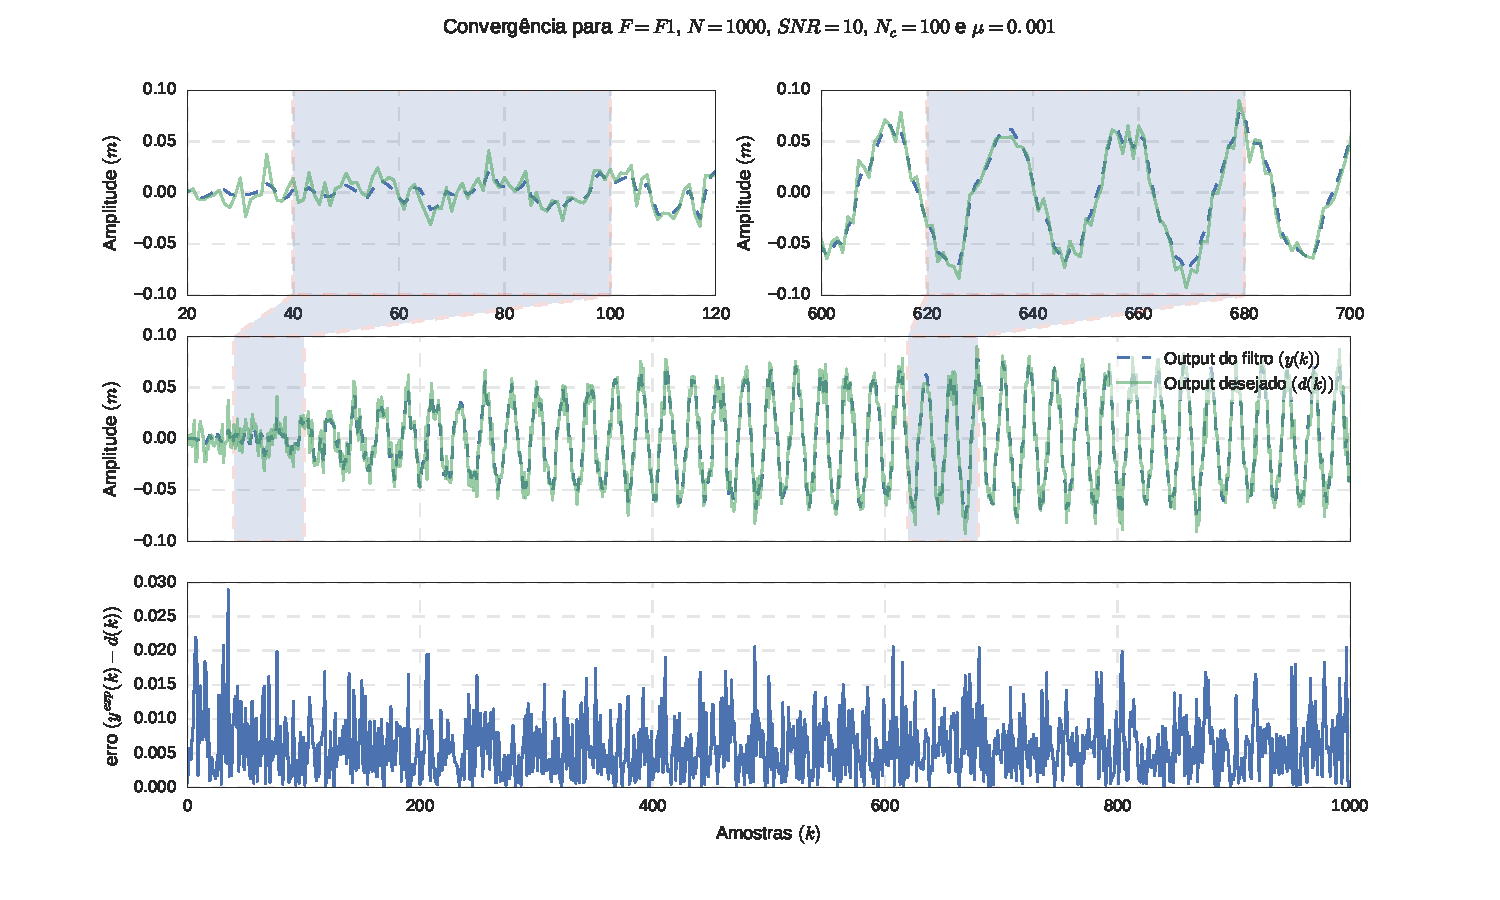
\includegraphics[scale=0.7]{F1_1000_10_conv}
	\caption{Evolução do filtro para $ F=F_1 $, $ N=1000 $ e $ SNR=10 $.}
	\label{fig:F1_1000_10_conv}
\end{figure}

Podemos tentar melhorar a adaptação aumentando o valor do fator de convergência de $ \mu=0.001 $ para $ \mu=0.003 $ o que por sua vez deve aumentar a velocidade de convergência do algoritmo. A \cref{fig:F1_1000_10_mu_003_conv} mostra que, quando utilizamos $ \mu = 0.003 $, o valor de saída do filtro tende a variar mais rapidamente tentando acompanhar o valor desejado, no entanto, as variações bruscas nos valores dos coeficientes do filtro não permitem a convergência e consequente minimização do erro após decorridas várias iterações. 

Conforme \citet{diniz1997adaptive}, o valor de $ \mu $ deve ser escolhido no intervalo mostrado na \cref{eq:mu}

\begin{equation}\label{eq:mu}
0 < \mu < \frac{1}{\lambda_{max}}
\end{equation}
onde $ \lambda_{max} $ corresponde ao maior autovalor da matriz $ {\bf R} $ definida na \cref{eq:mse2}. Podemos concluir que o valor $ \mu = 0.003 $ se encontra fora desse intervalo, já que a convergência não foi atingida e os resultados se apresentaram piores do que os obtidos com $ \mu=0.001 $. 

\begin{figure}
	\centering
	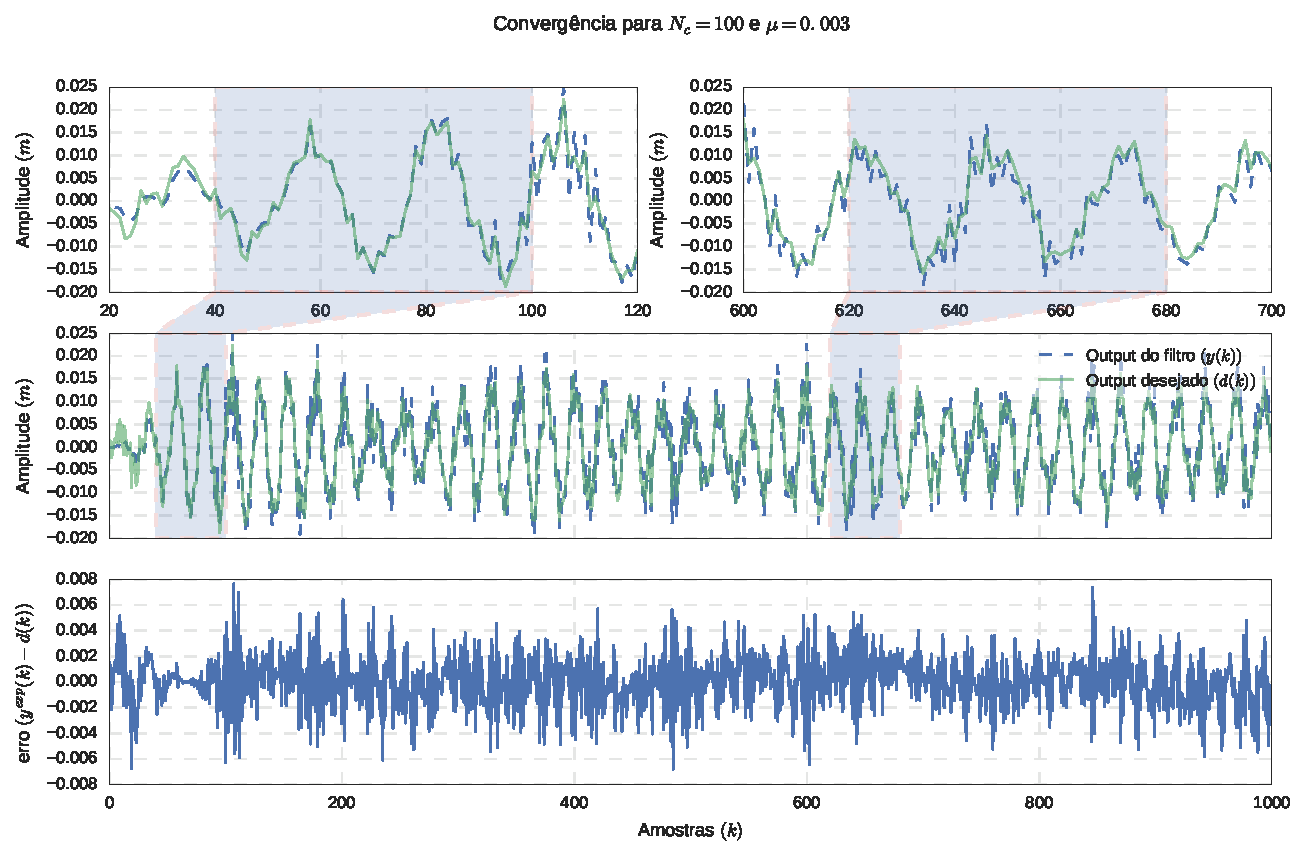
\includegraphics[scale=0.7]{F1_1000_10_mu_003_conv}
	\caption{Evolução do filtro para $ F=F_1 $, $ N=1000 $ e $ SNR=10 $.}
	\label{fig:F1_1000_10_mu_003_conv}
\end{figure}

Para que possamos obter melhores resultados iremos utiliza um fator maior que $ \mu=0.001 $ com o objetivo de aumentar a velocidade de adaptação do filtro e menor que $ \mu=0.003 $ para que a convergência possa ser obtida. A \cref{fig:F1_1000_10_mu_002_conv} mostra que para $ \mu=0.002 $ o filtro atinge a convergência rapidamente, apresentando valores de erro próximos de 0 após 100 iterações.

\begin{figure}
	\centering
	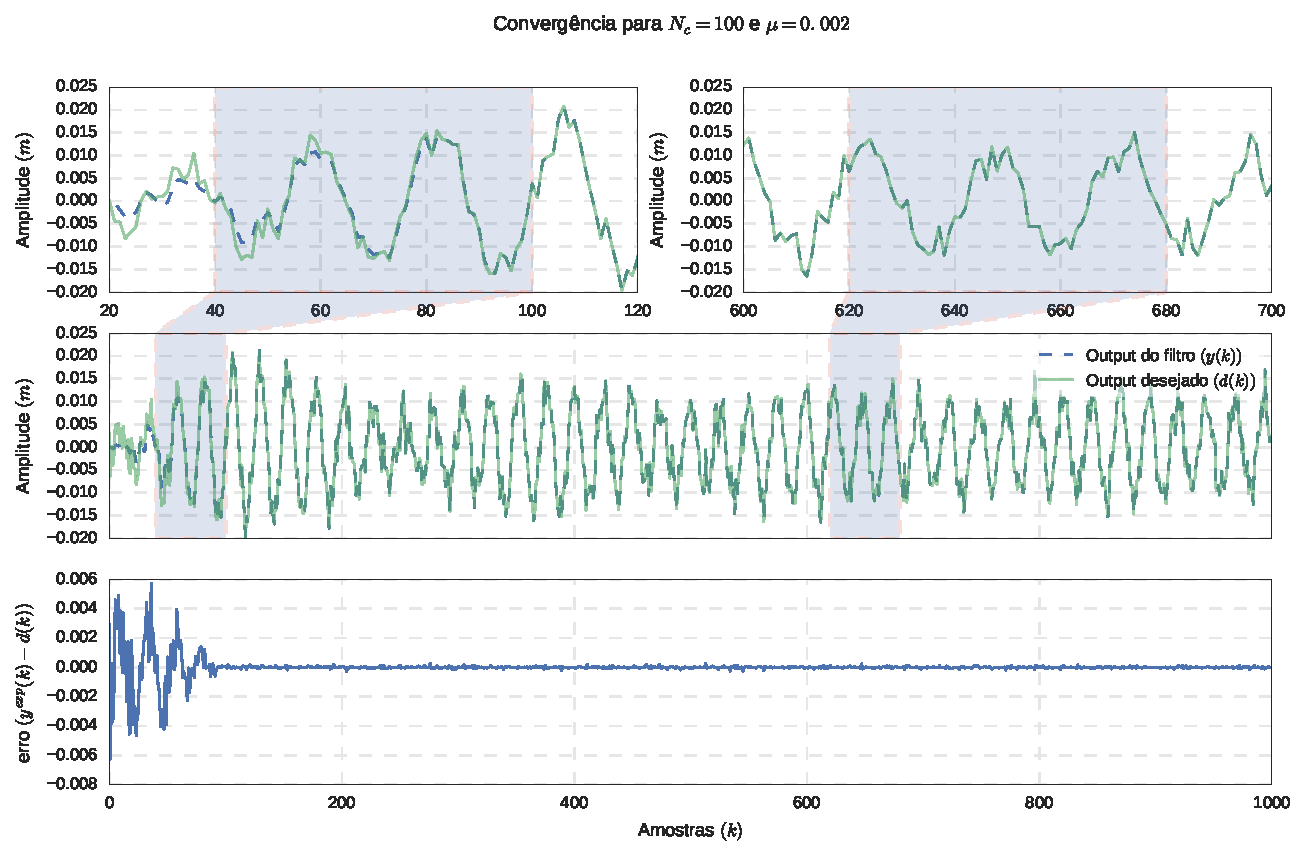
\includegraphics[scale=0.7]{F1_1000_10_mu_002_conv}
	\caption{Evolução do filtro para $ F=F_1 $, $ N=1000 $ e $ SNR=10 $.}
	\label{fig:F1_1000_10_mu_002_conv}
\end{figure}

\subsection{FRF do filtro}
Assim como visto em \ref{sec_F_0}, os resultados para as FRFs se mostraram muito parecidos utilizando-se o último vetor de coeficientes ou o valor esperado dos coeficientes tomando por base as observações da segunda metade do vetor de dados. Sendo assim, iremos apresentar a FRF apenas para o último vetor de coeficientes do filtro.

A \cref{fig:F1_1000_10_mu_002_FRF_med_False} mostra os resultados obtidos com $ N=1000 $ e $ SNR=90 $. Podemos notar uma melhora dos resultados quando comparamos com a FRF obtida para $ F=F_0 $, mas os valores ainda estão distantes da FRF real do sistema.

\begin{figure}
	\centering
	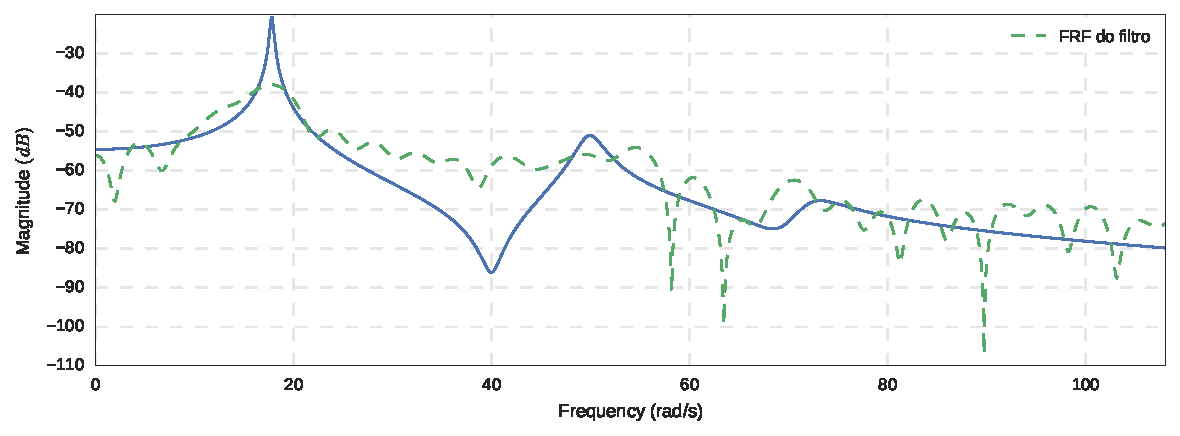
\includegraphics[scale=0.7]{F1_1000_10_mu_002_FRF_med_False}
	\caption{FRF do filtro obtido para $ F=F_1 $, $ N=1000 $ e $ SNR=10 $.}
	\label{fig:F1_1000_10_mu_002_FRF_med_False}
\end{figure}

\subsection{Predição}

Para a predição iremos utilizar a mesma força utilizada em $ F=F_0 $ e descrita na \ref{eq:F_3}. Os resultados da predição são apresentados na \cref{fig:F1_1000_10_mu_002_pred} e mostram uma melhora, mas podemos ver que este filtro também não foi capaz de prever de maneira precisa o comportamento do sistema para uma força diferente da utilizada no processo de adaptação.

\begin{figure}[h]
	\centering
	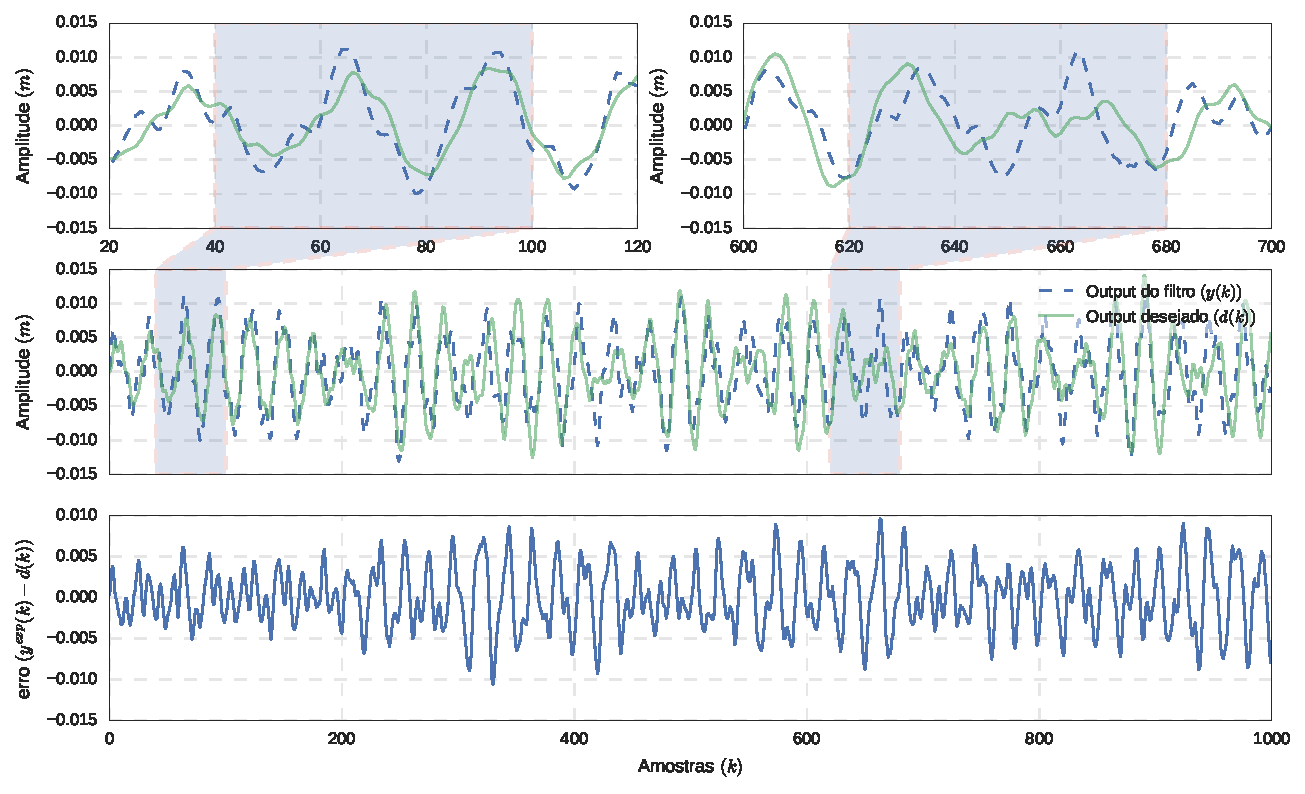
\includegraphics[scale=0.7]{F1_1000_10_mu_002_pred}
	\caption{Predição do filtro obtido com $ F=F_1 $, $ N=1000 $ e $ SNR=10 $.}
	\label{fig:F1_1000_10_mu_002_pred}
\end{figure}

\section{Resultados para $ F_2 $}
\subsection{Adaptação do filtro}

Os resultados da adaptação do filtro para uma força $ F_2 $ (ruído branco) com $ N=1000 $ são mostrados na \cref{fig:F2_1000_90_conv}, \cref{fig:F2_1000_50_conv} e \cref{fig:F2_1000_10_conv} para $ SNR = $ 90, 50 e 10  respectivamente. Neste caso, mesmo com o filtro possuindo 8 vezes mais coeficientes ($ Nc = $ 800), não foi possível obter a convergência.

A convergência só pode ser obtida para uma amostragem com $ N= $ 5000 e um filtro com 1800 coeficientes. Os resultados da adaptação para $ N= $ 5000 são mostrados na \cref{fig:F2_5000_90_conv}, \cref{fig:F2_5000_50_conv} e \cref{fig:F2_5000_10_conv} para $ SNR = $ 90, 50 e 10  respectivamente. Podemos observar que, mesmo para um nível de ruído elevado ($ SNR=10 $) o filtro apresentou uma boa convergência após aproximadamente 1600 iterações.

\begin{figure}
	\centering
	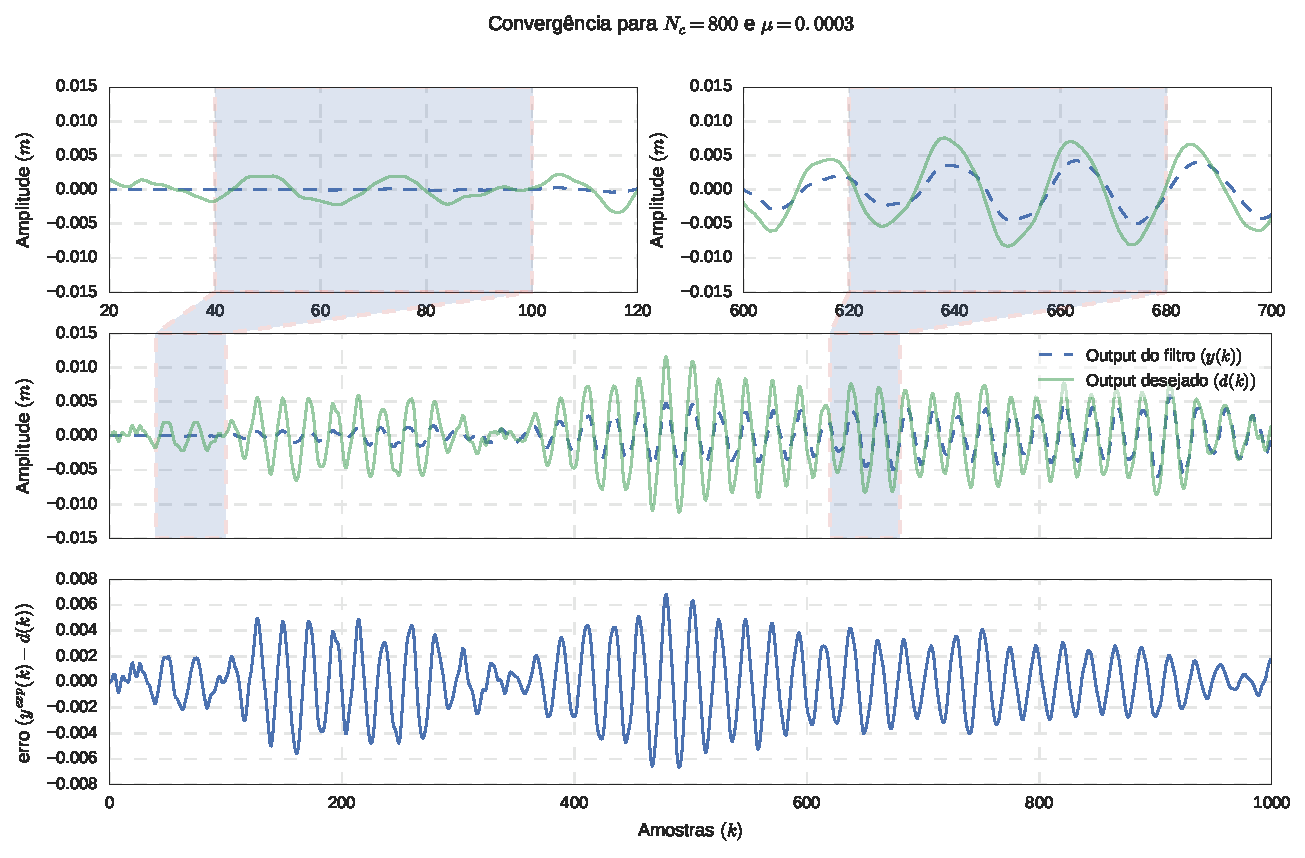
\includegraphics[scale=0.7]{F2_1000_90_conv}
	\caption{Evolução do filtro para $ F=F_2 $, $ N=1000 $ e $ SNR=90 $.}
	\label{fig:F2_1000_90_conv}
\end{figure}

\begin{figure}
	\centering
	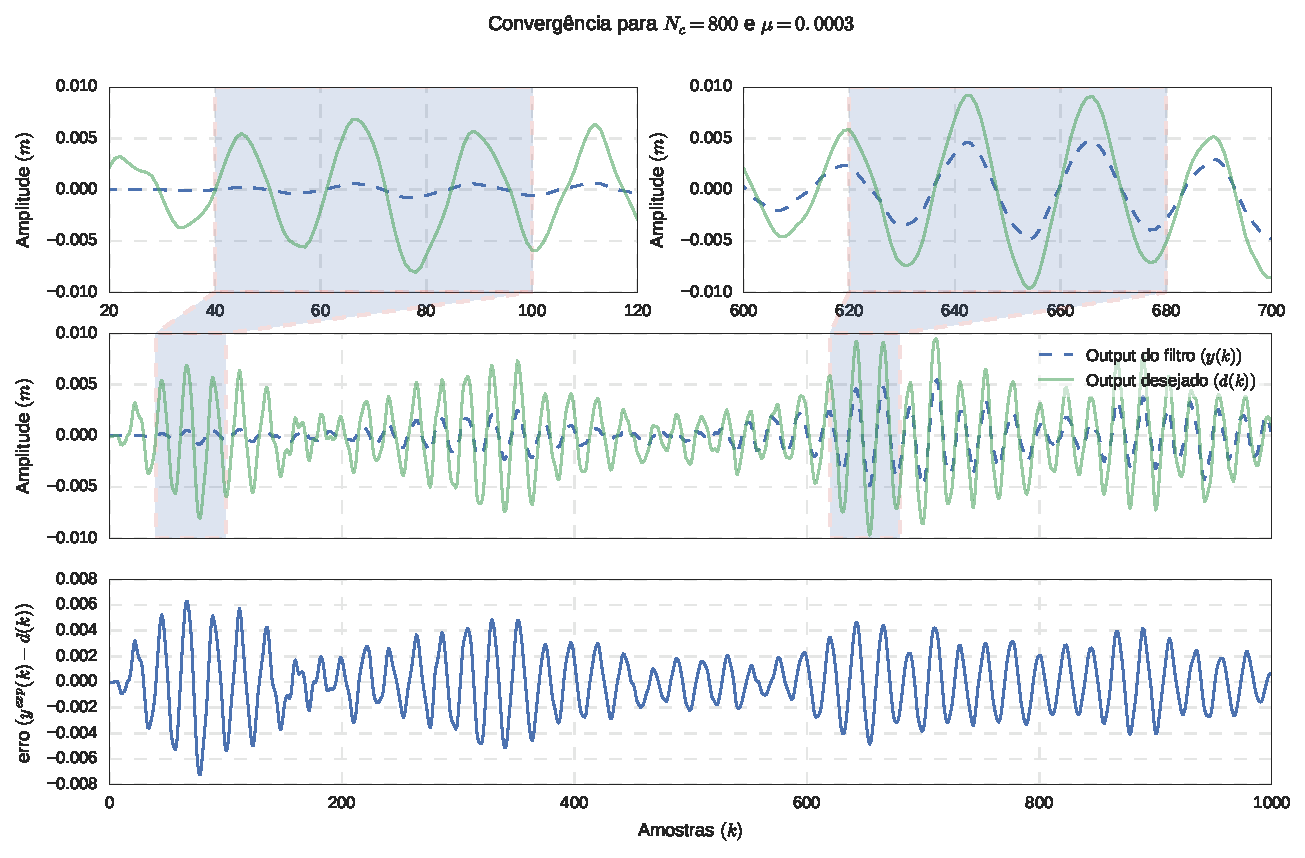
\includegraphics[scale=0.7]{F2_1000_50_conv}
	\caption{Evolução do filtro para $ F=F_2 $, $ N=1000 $ e $ SNR=50 $.}
	\label{fig:F2_1000_50_conv}
\end{figure}

\begin{figure}
	\centering
	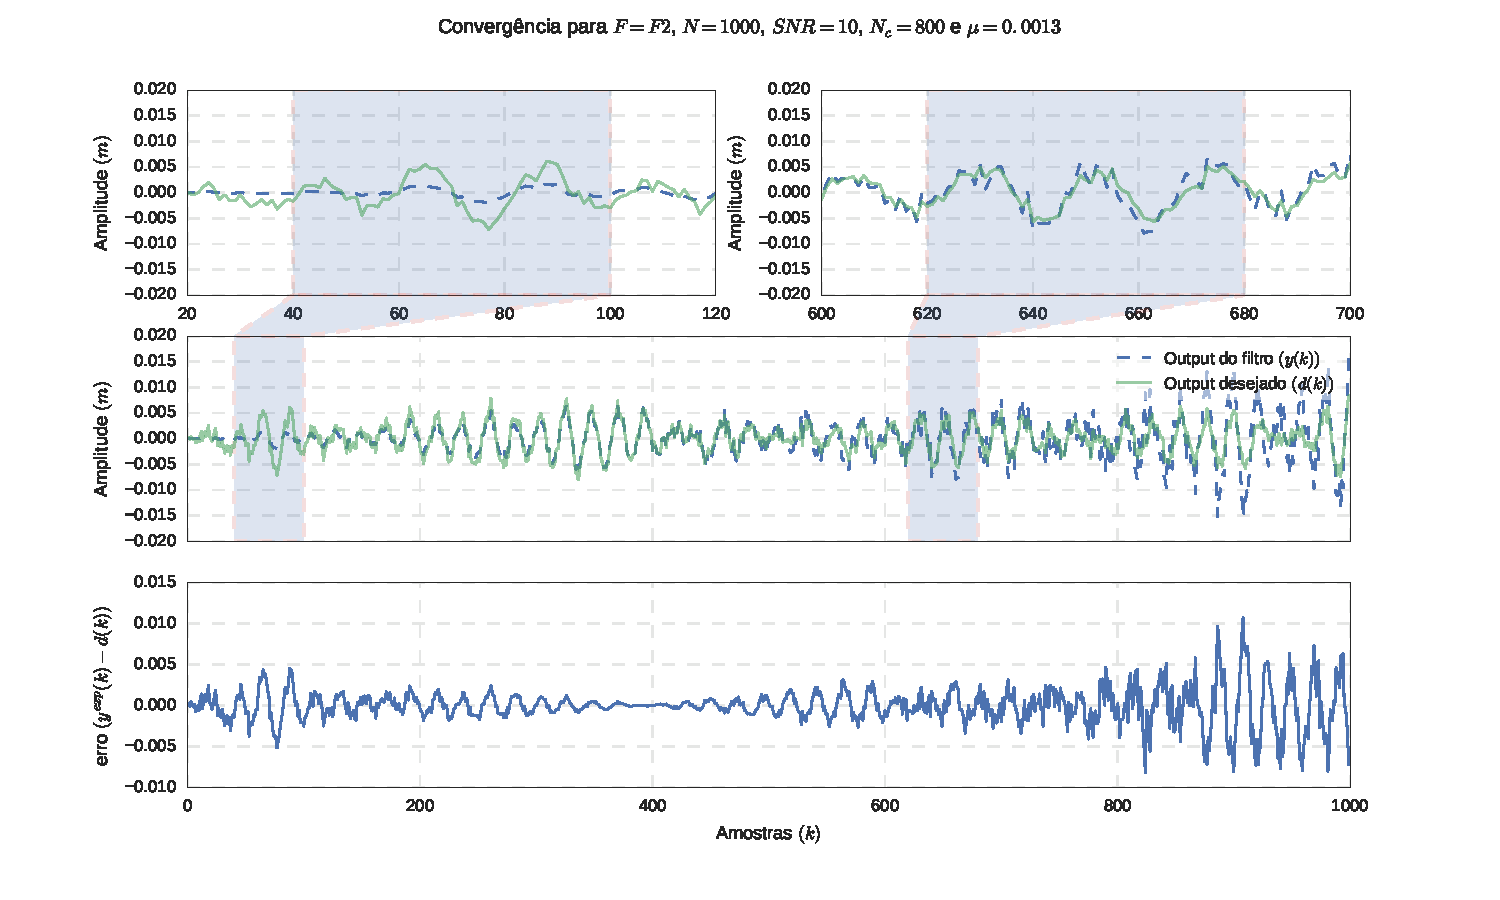
\includegraphics[scale=0.7]{F2_1000_10_conv}
	\caption{Evolução do filtro para $ F=F_2 $, $ N=1000 $ e $ SNR=10 $.}
	\label{fig:F2_1000_10_conv}
\end{figure}

\begin{figure}
	\centering
	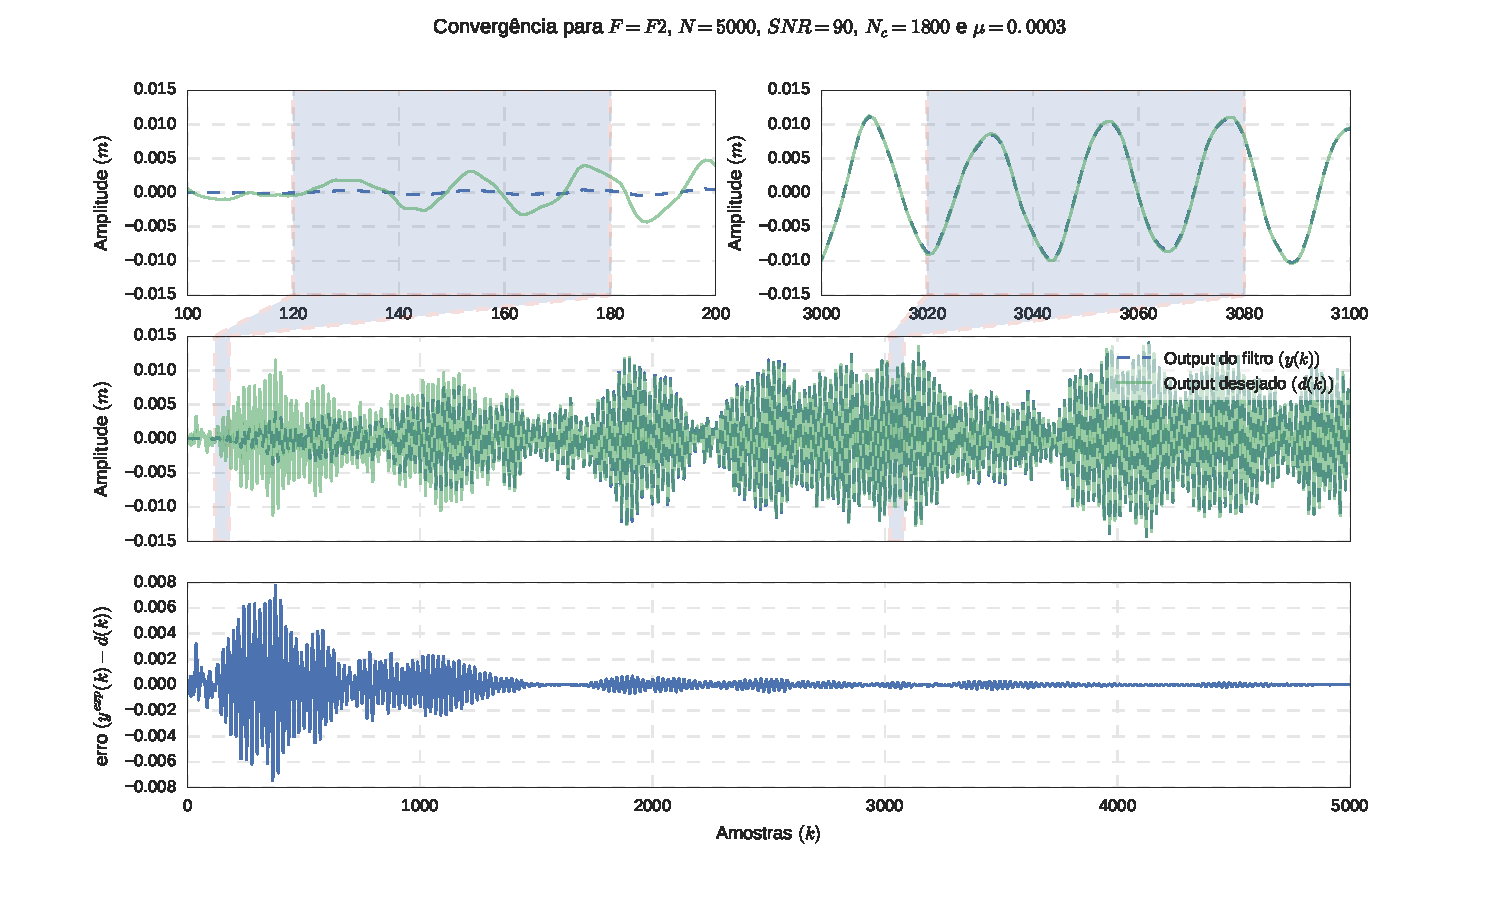
\includegraphics[scale=0.7]{F2_5000_90_conv}
	\caption{Evolução do filtro para $ F=F_2 $, $ N=5000 $ e $ SNR=90 $.}
	\label{fig:F2_5000_90_conv}
\end{figure}

\begin{figure}
	\centering
	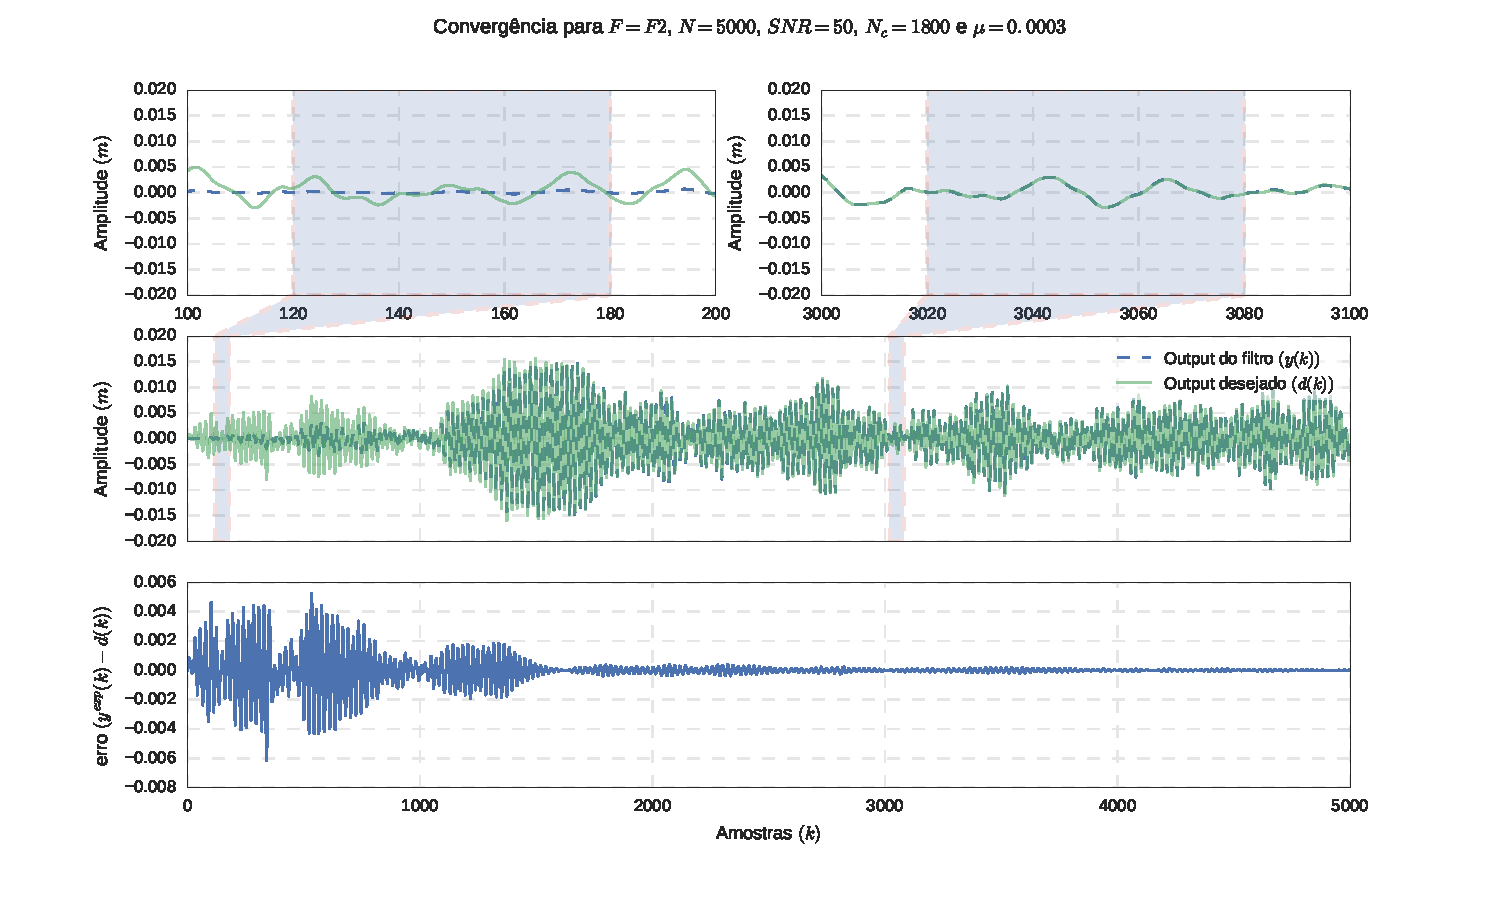
\includegraphics[scale=0.7]{F2_5000_50_conv}
	\caption{Evolução do filtro para $ F=F_2 $, $ N=5000 $ e $ SNR=50 $.}
	\label{fig:F2_5000_50_conv}
\end{figure}

\begin{figure}
	\centering
	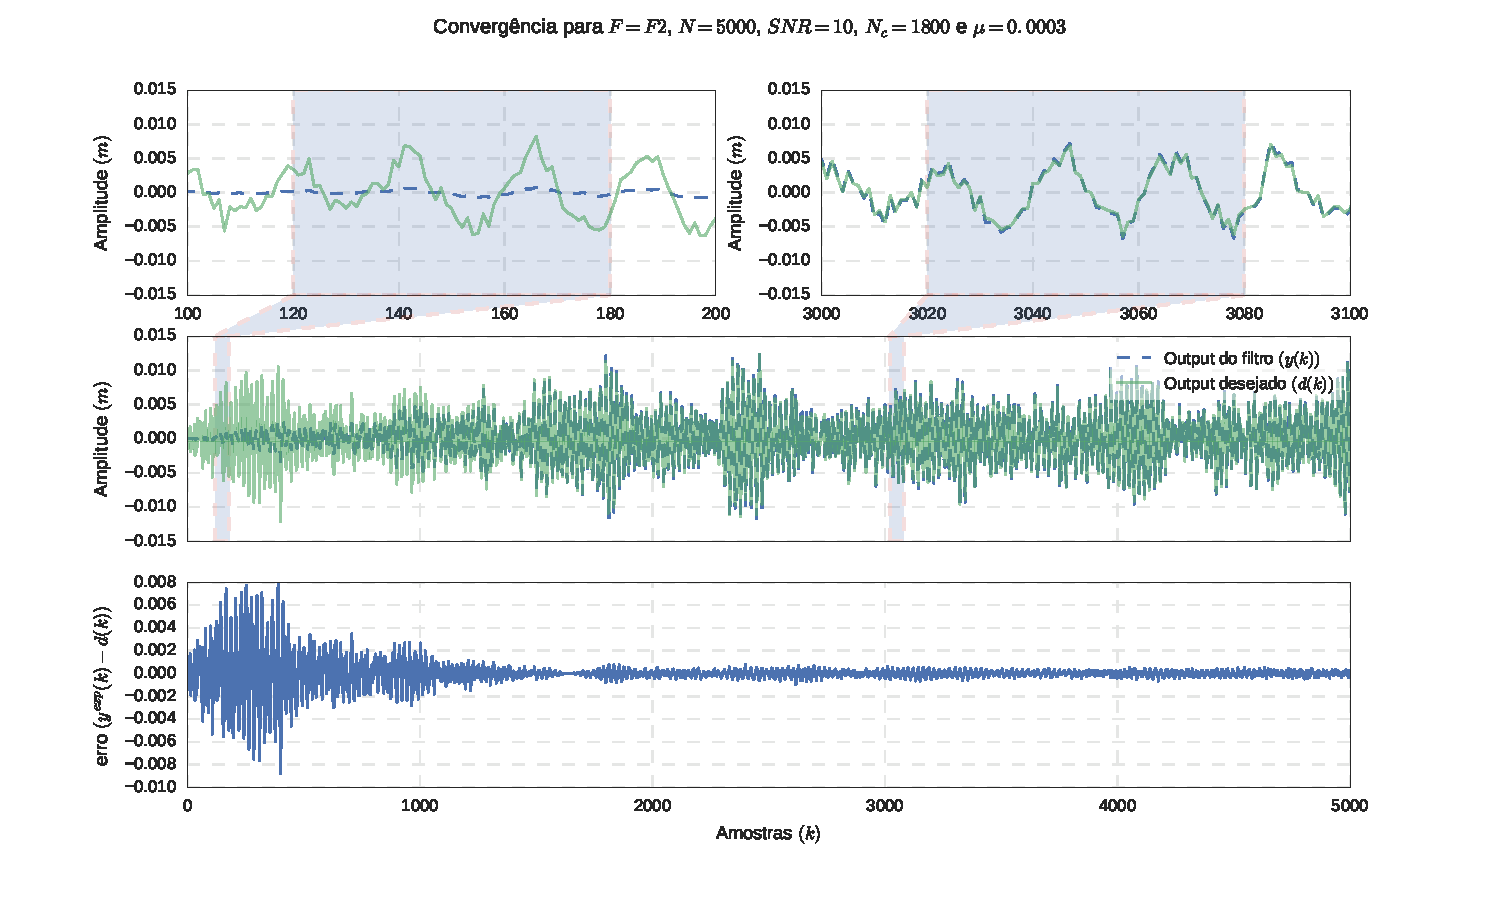
\includegraphics[scale=0.7]{F2_5000_10_conv}
	\caption{Evolução do filtro para $ F=F_2 $, $ N=5000 $ e $ SNR=10 $.}
	\label{fig:F2_5000_10_conv}
\end{figure}

\subsection{FRF do filtro}
Para a análise das FRFs iremos utilizar os filtros obtidos com $ N=5000 $, já que apenas estes apresentaram convergência nos seus coeficientes. Além disso, assim como na análise de $ F_1 $, apenas as FRFs do último vetor de coeficientes do filtro serão apresentadas.

\begin{figure}
	\centering
	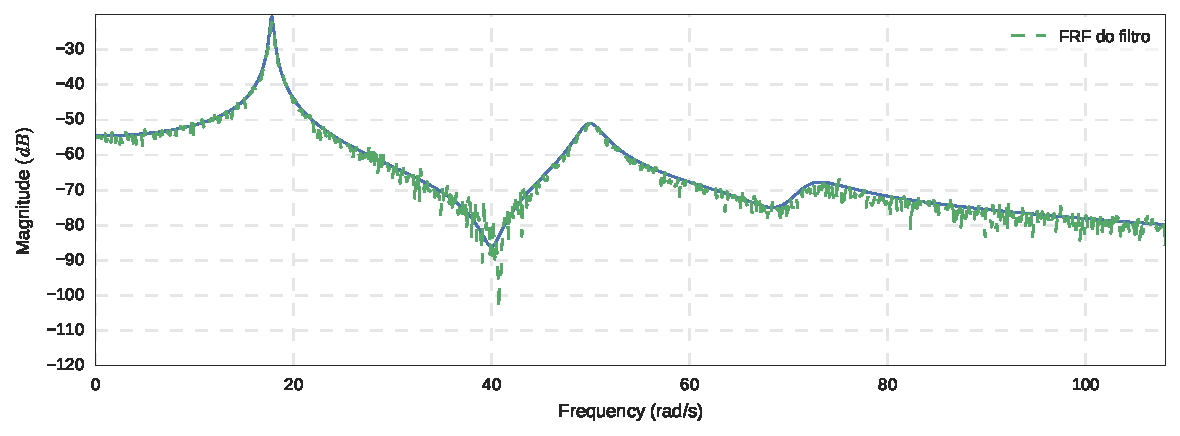
\includegraphics[scale=0.7]{F2_5000_90_FRF_med_False}
	\caption{FRF do filtro obtido para $ F=F_2 $, $ N=5000 $ e $ SNR=90 $.}
	\label{fig:F2_5000_90_FRF_med_False}
\end{figure}

A \cref{fig:F2_5000_90_FRF_med_False} mostra que para $ SNR=90 $ a FRF do filtro apresenta excelentes resultados quando comparada à FRF real do sistema. Os três picos referente às frequências naturas foram capturados, além disso a queda na amplitude devido o fenômeno de anti-ressonância também é claramente observado. Outro ponto importante é que, mesmo nas frequências mais elevadas e distantes das frequências naturais, a FRF do filtro reproduziu com exatidão os valores de amplitude esperados.

\begin{figure}
	\centering
	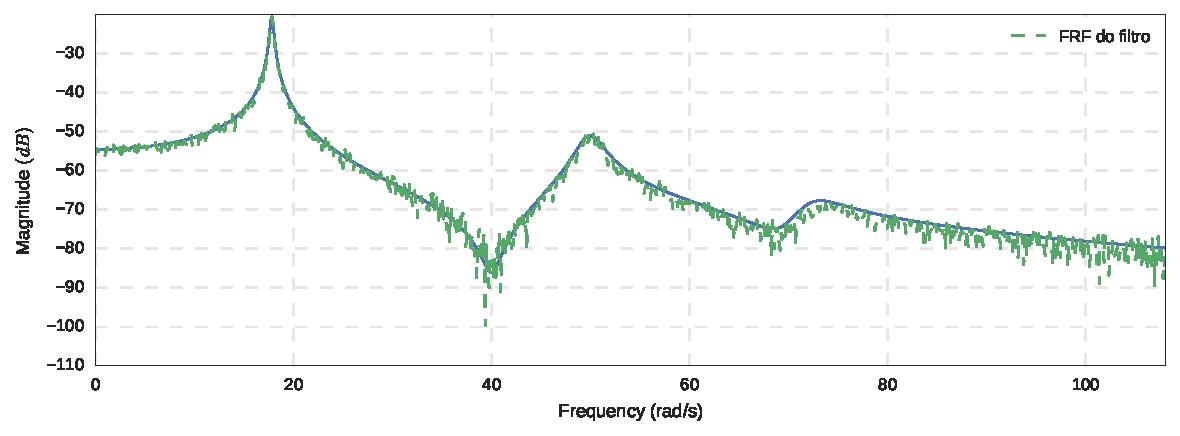
\includegraphics[scale=0.7]{F2_5000_50_FRF_med_False}
	\caption{FRF do filtro obtido para $ F=F_2 $, $ N=5000 $ e $ SNR=50 $.}
	\label{fig:F2_5000_50_FRF_med_False}
\end{figure}

A \cref{fig:F2_5000_50_FRF_med_False} mostra que, para $ SNR=50 $, os resultados ainda são satisfatórios. No entanto, ao aumentarmos o nível de ruído no sinal, podemos notar que para frequências mais elevadas a FRF do filtro apresenta uma maior variação, diferindo um pouco dos valores esperados quando comparamos com a FRF do sistema.

\begin{figure}
	\centering
	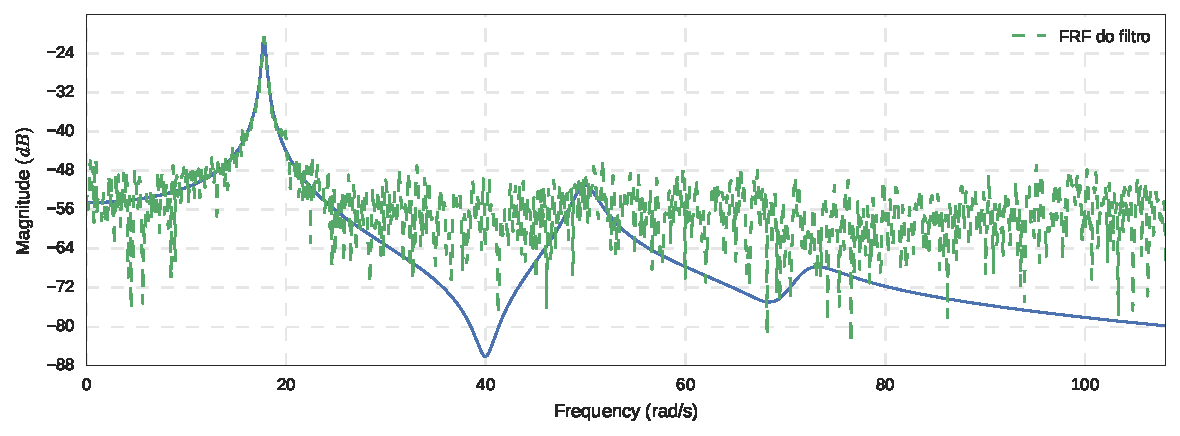
\includegraphics[scale=0.7]{F2_5000_10_FRF_med_False}
	\caption{FRF do filtro obtido para $ F=F_2 $, $ N=5000 $ e $ SNR=10 $.}
	\label{fig:F2_5000_10_FRF_med_False}
\end{figure}

A \cref{fig:F2_5000_10_FRF_med_False} apresenta a FRF para nível de ruído com $ SNR=10 $. Neste caso ainda foi possível obter um bom resultado para a primeira frequência natural, mas se afastando desse pico vemos que o filtro não descreve bem o sistema. O fenômeno de anti-ressonância não é observado e mesmo o pico referente à segunda frequência natural não pode ser visto claramente.

\subsection{Predição}

\begin{figure}
	\centering
	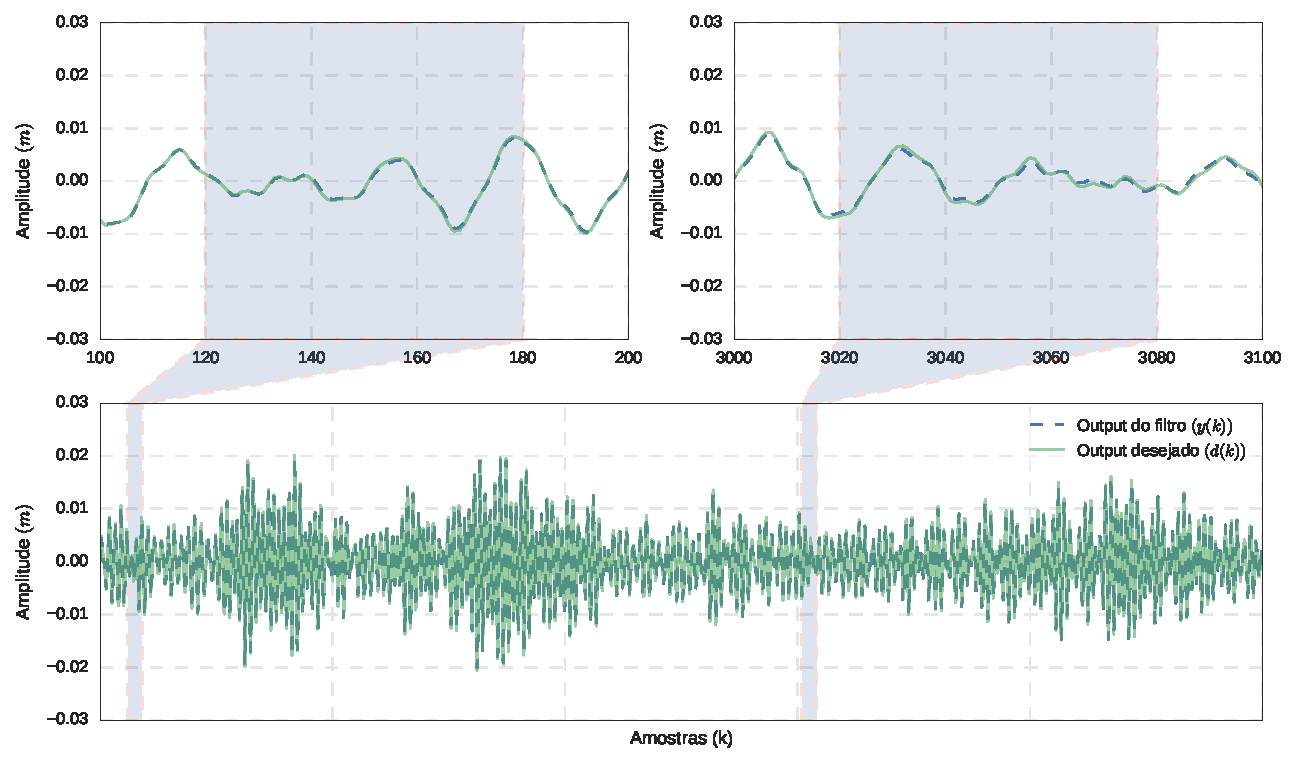
\includegraphics[scale=0.7]{F2_5000_90_pred}
	\caption{Predição do filtro obtido com $ F=F_2 $, $ N=5000 $ e $ SNR=90 $.}
	\label{fig:F2_5000_90_pred}
\end{figure}

Para a predição iremos utilizar a mesma força utilizada em $ F=F_0 $ e descrita na \ref{eq:F_3}. Os resultados da predição são apresentados na \cref{fig:F2_5000_90_pred} e na \cref{fig:F2_5000_10_pred}, para $ SNR= $ 90 e 10 respectivamente. Os resultados mostram que, para $ SNR=10 $, o filtro obtido é capaz de prever com grande exatidão a resposta do sistema.  

\begin{figure}
	\centering
	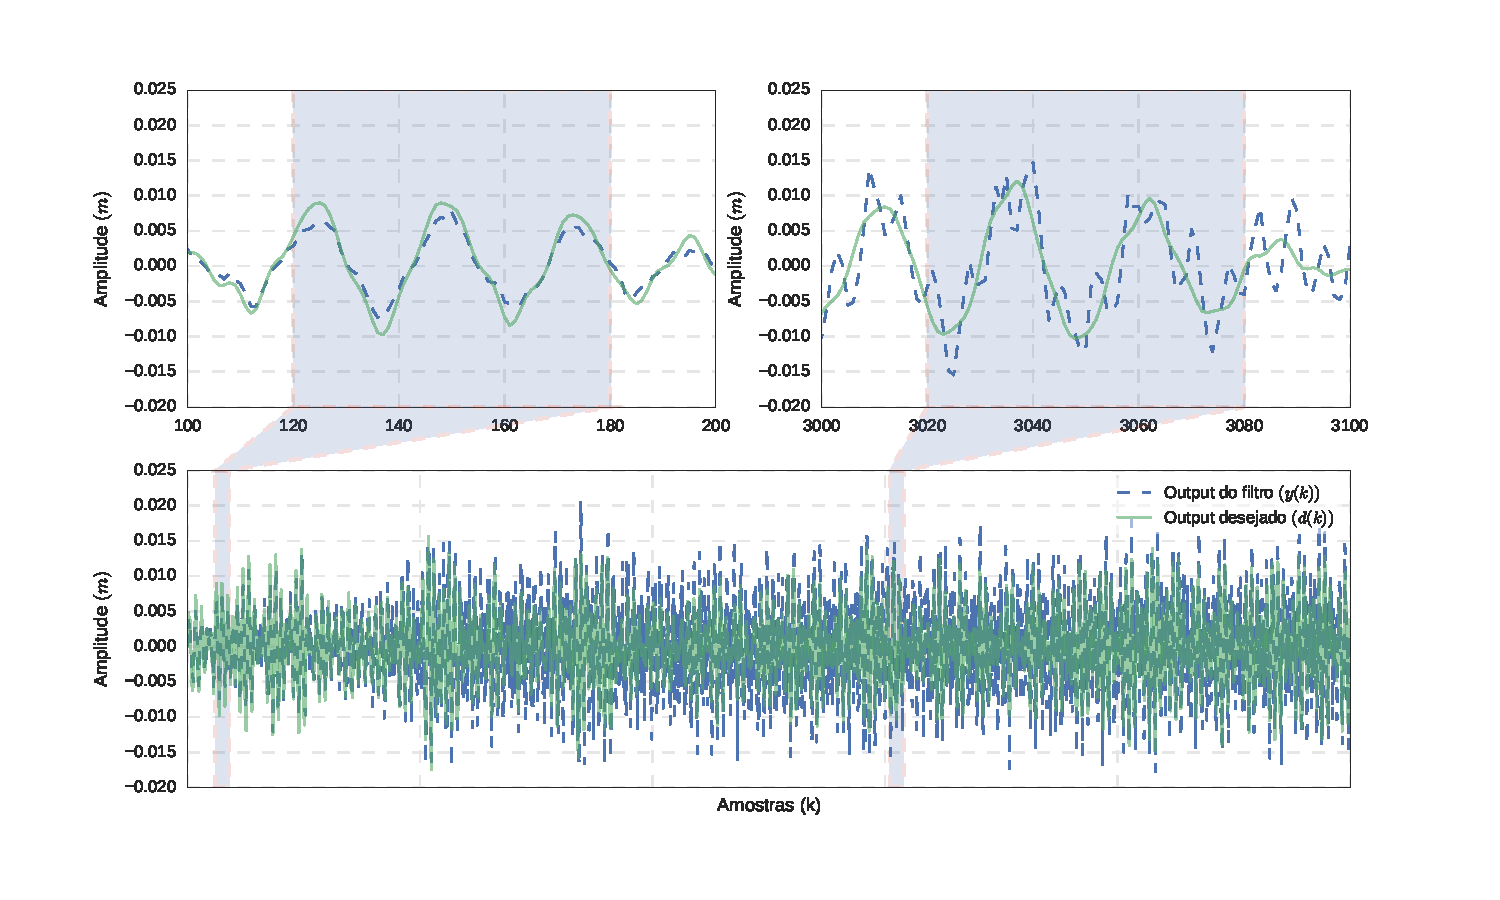
\includegraphics[scale=0.7]{F2_5000_10_pred}
	\caption{Predição do filtro obtido com $ F=F_2 $, $ N=5000 $ e $ SNR=10 $.}
	\label{fig:F2_5000_10_pred}
\end{figure}

  \chapter{Conclusões}


  \backmatter
  \bibliographystyle{coppe-unsrt}
  \bibliography{thesis}

  \appendix
  \chapter{Código utilizado}

Foi omitido o código utilizado para gerar o sistema utilizado (código do trabalho 1) e para plotar os gráficos apresentados no trabalho.

\begin{minted}{python3}


def F0(t):
	A0 = 1
	w0 = 33.84
	return A0*np.sin(w0*t)

def F1(t):
	A1, A2 = (1, 2)
	w1, w2 = (0.9*18, 1.1*50)
	return A1*np.sin(w1*t) + A2*np.sin(w2*t)

def F2(t):
	var = 1
	norm = stats.norm(0, np.sqrt(var))
	return norm.rvs(len(t))

def F4(t):
	A1, A2, A3 = (1, 2, 3)
	w1, w2, w3 = (0.7*20, 0.8*50, 1.3*50)
	var = 1
	norm = stats.norm(0, np.sqrt(var))
	return A1*np.sin(w1*t) + A2*np.sin(w2*t) + A3*np.sin(w3*t) + norm.rvs(len(t))
	
m0, m1, m2 = (1, 1, 1)
k0, k1, k2 = (1600, 1600, 1600)
M1 = np.array([[m0, 0, 0],
		[0, m1, 0],
		[0, 0, m2]])
K1 = np.array([[k0+k1, -k1,   0],
		[-k1, k1+k2, -k2],
		[0,     -k2,  k2]])
alpha, beta = 1e-3, 1e-3
C1 = alpha*M1 + beta*K1
sys = vt.VibSystem(M1, alpha*M1 + beta*K1, K1,
r'Sistema 1 - $\alpha = 10^{-3}$ e $\beta = 10^{-3}$')

def noise(sig, snr):
	"""
	Returns a corrupted signal based on a
	signal-to-noise ratio (SNR).
	"""
	a_s = np.sqrt((sig * sig).mean())
	a_n = a_s/10**(snr/20)
	var = a_n**2
	norm = stats.norm(0, np.sqrt(var))
	
	return sig + norm.rvs(len(sig))


class LMSFilter(object):
	def __init__(self, Nc, mu):
		"""
		Iniciar filtro com Nc coeficientes.
		"""
		self.Nc = Nc
		self.mu = mu
		# valores iniciais para o filtro w = [0, 0, ..., 0]
		self.w = np.zeros(Nc)
	
	def predict(self, x):
		y = self.w @ x
		return y
	
	def update(self, d, x):
		"""
		Atualizar filtro baseado no sinal de entrada x
		e no valor desejado d.
		"""
		y = self.w @ x
		e = d - y
		self.w += 2 * self.mu * e * x
		
class SysId(object):
	def __init__(self, name, sys, Nc, mu, F, N, snr,
	inp=2, out=0):
	self.name = name
	self.names = name.split('_')
	self.sys = sys
	self.Nc = Nc
	self.mu = mu
	self.F = F
	self.N = N
	self.snr = snr
	self.inp = inp
	self.out = out
	
	# criar filtro
	self.filt = vt.LMSFilter(Nc, mu)
	
	# criar array de tempo
	self.dt = 1/(8*(50/(2*np.pi)))
	self.t = np.linspace(0, N*self.dt, N)
	
	# criar forçamento (input)
	F_ = np.zeros((len(self.t), sys.n))
	F_[:, inp] = F(self.t)
	self.F_ = F_
	self.x = F_[:, inp]
	
	# resposta do sistema (d)
	_, _, self.sys_time_resp = sys.time_response(self.F_, self.t)
	self.d = self.sys_time_resp[:, out] # selecionar output
	
	# resposta do sistema com ruído (d_noise)
	d_n = np.copy(self.sys_time_resp.T)
	for i, sig in enumerate(d_n):
	d_n[i, :] = noise(sig, snr)
	self.sys_time_resp_noise = d_n.T
	self.d_noise = self.sys_time_resp_noise[:, out] # sel. output
	
	# atualizar filtro
	ws_hist = np.zeros((N, Nc))
	ys_hist = np.zeros(N)
	# adicionar Nc zeros ao início do input
	self.x_shift = np.concatenate([np.zeros(Nc - 1), self.x])
	for i in range(N):	
		self.filt.update(self.d_noise[i], self.x_shift[i: i + Nc])
		ys_hist[i] = self.filt.predict(self.x_shift[i: i + Nc])
		ws_hist[i] = self.filt.w

	self.w = self.filt.w
	self.ws = ws_hist
	self.ys = ys_hist
	self.e = ((self.d_noise - self.ys))
	
	def y_last_w(self, sig):
		N = self.N
		Nc = self.Nc
		sig = np.concatenate([np.zeros(Nc - 1), sig])
		y_last_w = np.zeros(N)
		for i in range(N):
		y_last_w[i] += self.filt.predict(sig[i: i + Nc])
	
	return y_last_w
	
	def freq_resp(self, sig, worN):
		fs = 1/self.dt
		w, h = signal.freqz(sig, worN=worN)
		w *= fs

	return w, h

\end{minted}

\end{document}
